\documentclass[12pt,a4paper,twoside]{article}
% Change "article" to "report" to get rid of page number on title page
\usepackage{amsmath,mathtools,amsfonts,amsthm,amssymb}
\usepackage{setspace}
\usepackage{Tabbing}
\usepackage{cite}
\usepackage{fancyhdr}
\usepackage{lastpage}
\usepackage{extramarks}
\usepackage{chngpage}
\usepackage{fourier}
\usepackage{soul,color}
\usepackage[usenames,dvipsnames]{xcolor}
\usepackage{graphicx,float,wrapfig}
\usepackage[utf8]{inputenc}
\usepackage{sidecap}
\usepackage{marvosym}
\usepackage{tikz, tikz-qtree}
\usepackage{tabularx, multirow}
\usepackage{enumerate}
\usepackage{hyperref}
\usepackage{cleveref}
\usepackage{zref}
\usepackage{pgffor}
\definecolor{gray99}{gray}{.99}
\usepackage{listings}
\usepackage[english]{babel}
\usepackage{placeins}
\usepackage{tikz}
\usepackage{tikz-qtree}
\usepackage{xspace}
\usepackage{mathtools}
\usepackage{tabulary}
\lstset{
	language=Matlab,
	backgroundcolor=\color{gray99},
	tabsize=3,
	frame=single,
	keywordstyle=\ttfamily\bfseries\color{RoyalBlue},
	commentstyle=\ttfamily\color{ForestGreen},
	stringstyle=\ttfamily\color{Gray},
	breaklines=true,
	showstringspaces=false,
	basicstyle=\small\ttfamily,
	emph={label},
	xleftmargin=22pt,
	framexleftmargin=22pt,
	framexrightmargin=0pt,
	framexbottommargin=4pt,
	numbers=left,
	stepnumber=1
}
\usepackage{caption}
\usepackage{xstring}
\DeclareCaptionFont{black}{\color{black}}{\bfseries}
\DeclareCaptionFormat{listing}{\parbox{\textwidth}{\hspace{8pt}#1#2#3}}
\captionsetup[lstlisting]{format=listing,labelfont=black,textfont=black, singlelinecheck=false, margin=0pt, font={bf,footnotesize}}

% In case you need to adjust margins:
\topmargin=-0.45in      %
\evensidemargin=0in     %
\oddsidemargin=0in      %
\textwidth=6.5in        %
\textheight=9.5in       %
\headsep=0.25in         %

% Homework Specific Information
\newcommand{\hmwkTopic}{Automatic Material Recognition Using Computer Vision}
\newcommand{\hmwkTitle}{\hmwkTopic}
\newcommand{\hmwkDueDate}{\today}
\newcommand{\hmwkClass}{Trabajo Final de Grado}
\newcommand{\hmwkDegree}{Grado en Ingeniería Informática}
\newcommand{\hmwkYear}{Curso 2013 / 2014}
\newcommand{\hmwkSchool}{Escola Tècnica Superior d’Enginyeria Informàtica}
\newcommand{\hmwkUniversity}{Universitat Politècnica de València}
\newcommand{\hmwkAuthorNameA}{David A. Forsyth}
\newcommand{\hmwkAuthorEmailA}{daf@illinois.edu}
\newcommand{\hmwkAuthorNameB}{Roberto Paredes}
\newcommand{\hmwkAuthorEmailB}{rparedes@dsic.upv.es}
\newcommand{\hmwkAuthorNameC}{José Vicente Ruiz Cepeda}
\newcommand{\hmwkAuthorEmailC}{josruice@upv.es}

% Setup the header and footer
\pagestyle{fancy}                                                       %
% \lhead{\hmwkAuthorNameC}                                                 %
% \chead{}  %
% \rhead{\hmwkTopic}     
%                                                 %
% \lfoot{}                                                %
% \cfoot{\hyperlink{toc}{\thepage}}%
% \rfoot{}                          %

\fancyhead[L,R,C]{}
\fancyhead[LO]{\small\hmwkAuthorNameC}
\fancyhead[RE]{\small\hmwkTopic}
\fancyfoot[L,R,C]{}
\fancyfoot[RO,LE]{\small\hyperlink{toc}{\thepage}}

\renewcommand{\headrulewidth}{0pt}% disable the underline of the header part

% \renewcommand\headrulewidth{0.4pt}                                      %
% \renewcommand\footrulewidth{0.4pt}                                      %


%%%%%%%%%%%%%%%%%%%%%%%%%%%%%%%%%%%%%%%%%%%%%%%%%%%%%%%%%%%%%
% Make title
\title{
    \vspace{-1in}
    \begin{figure}[ht!]
        \centering
        \begin{minipage}{0.42\textwidth}
            \centering
            
\includegraphics[width=\textwidth]{Images/UPV.png}
        \end{minipage}    
        \hspace{0.15\textwidth}
        \begin{minipage}{0.42\textwidth}
            \centering
            
\includegraphics[width=\textwidth]{Images/ETSINF.png}
        \end{minipage}
    \end{figure}
    \vspace{0.5in}
    \textcolor{gray}{\Large\hmwkSchool} \\
    \textcolor{gray}{\Large\hmwkUniversity} \\
    \vspace{1.2in}
    \textmd{\textbf{\huge\hmwkTitle}}\\
    \vspace{0.3in}
    \large\hmwkClass \\
    \vspace{0.15in}
    \Large\hmwkDegree
    \vspace{2.5in}
}
\date{}
\author{
	\begin{minipage}{0.48\textwidth}
		\vspace{-3cm}
		\centering
		{\small UIUC advisor \\}
		\textbf{\hmwkAuthorNameA} \\\small<\texttt{\href{mailto:daf@illinois.edu}{\hmwkAuthorEmailA}}> 
	\end{minipage}
	\begin{minipage}{0.48\textwidth}
		\vspace{-3cm}
		\centering
		{\small UPV advisor \\}
		\textbf{\hmwkAuthorNameB} \\\small<\texttt{\href{mailto:rparedes@dsic.upv.es}{\hmwkAuthorEmailB}}>
	\end{minipage} \\\\\\
	\begin{minipage}{0.48\textwidth}
		\vspace{-1.5cm}
		\centering
		{\small Student \\}
		\textbf{\hmwkAuthorNameC} \\\small<\texttt{\href{mailto:josruice@upv.es}{\hmwkAuthorEmailC}}>
	\end{minipage} \\\\\\
    \textcolor{gray}{\large\hmwkYear}
}
%%%%%%%%%%%%%%%%%%%%%%%%%%%%%%%%%%%%%%%%%%%%%%%%%%%%%%%%%%%%%

\begin{document}
\begin{singlespace}

\begin{titlepage}
\maketitle
\thispagestyle{empty}
\newpage\null\thispagestyle{empty}\newpage % Empty page after title.
\end{titlepage}


% Abstract.
\section*{Resumen}
\emph{La habilidad de identificar los materiales de los objetos del mundo real es clave para los seres humanos. Por ello, un sistema automático con esta capacidad sería un gran paso en el camino hacia la simulación de la visión humana. Este trabajo describe una nueva aproximación para intentar resolver este problema aún abierto, donde la idea clave es el uso de propiedades inferibles a través de las imágenes como paso intermedio para reconocer materiales.} \\

\emph{El algoritmo se basa en la extracción y cuantización de descriptores \emph{SIFT}, que son usados para entrenar \emph{SVMs} en el reconocimiento de propiedades de los materiales, tanto táctiles como de forma, en diferentes escalas. Finalmente, modelos basados en \emph{Naive Bayes} y \emph{SVMs} son entrenados y comparados para clasificar materiales a partir de las propiedades. A pesar del alto costo del marcado, esta aproximación ofrece interesantes resultados intermedios y precisión competitiva con otros métodos utilizados sobre el mismo conjunto de imágenes.} \\

\textbf{Palabras clave:} Vision por Computador, reconocimiento de materiales, SVM, SIFT.

\vspace{2cm}

\section*{Abstract}
\emph{The ability to correctly identify the materials of objects in the real world is key in human's life. Therefore, an automatic system with that skill would be a great step in the path to simulate human vision. This work describes a new approach to try to solve this still open problem where the key idea is the use of image-inferable properties as an intermediate step to recognize materials.} \\

\emph{The algorithm is based on the extraction and quantization of \emph{SIFT} descriptors, which are later used to train \emph{SVMs} to recognize material properties, both of touch and shape, at different scales. Finally, models based on \emph{Naive Bayes} and \emph{SVMs} are trained and compared in terms of material recognition from the properties. Despite of the high cost of the markup, this approach offers interesting intermediate results and competitive accuracy compared with other methods applied to the same image dataset.} \\

\textbf{Keywords:} Computer Vision, material recognition, SVM, SIFT. 

\clearpage

% Uncomment the \tableofcontents and \newpage lines to get a Contents page
% Uncomment the \setcounter line as well if you do NOT want subsections
%       listed in Contents
%\setcounter{tocdepth}{1}
\hypertarget{toc}{}
\tableofcontents
\newpage

% When problems are long, it may be desirable to put a \newpage or a
% \clearpage before each homeworkProblem environment


\clearpage

% Own commands:
\newcommand{\checkEmpty}[3]{
    \normalexpandarg
    \exploregroups
    \IfStrEq{#1}{}{#2}{#3}
}

\newcommand{\datasetPath}{../../Dataset}

\newcommand{\e}[1]{\emph{#1}\xspace}

\crefformat{footnote}{#2\footnotemark[#1]#3} % Required for footnotes with href.

\newcommand{\imageSizeSingle}{0.30}
\newcommand{\dataSizeSingle}{0.65}
\newcommand{\spaceSizeSingle}{0.02}
\newcommand{\inputImage}[8]{
\begin{figure}[!ht]
    \centering
    \begin{minipage}{\imageSizeSingle\textwidth}
        \centering
        \includegraphics[width=\textwidth]{../../Dataset/\matName/\imgNumber.png}
    \end{minipage}
    \hspace{\spaceSizeSingle\textwidth}
    \begin{minipage}{\dataSizeSingle\textwidth}
        \textbf{\large \matName \xspace \imgNumber}:

        #7
        \begin{itemize}
            \item \textbf{Fine}: #1, #2.
            \item \textbf{Medium}: #3, #4.
            \item \textbf{Coarse}: #5, #6.
        \end{itemize}
        #8
    \end{minipage}
\end{figure}
\FloatBarrier    
}

\newcommand{\imageSizeDouble}{0.45}
\newcommand{\spaceSizeDouble}{0.05}
\newcommand{\plotTwoImages}[8]{
    \begin{figure}[!ht]
        \centering
        \begin{minipage}{\imageSizeDouble\textwidth}
            \centering
            \includegraphics[width=\textwidth]{#1}
            \checkEmpty{#2}{}{\caption{#2}}
            \label{#3}
        \end{minipage}
        \hspace{\spaceSizeDouble\textwidth}
        \begin{minipage}{\imageSizeDouble\textwidth}
            \centering
            \includegraphics[width=\textwidth]{#4}
            \checkEmpty{#5}{}{\caption{#5}}
            \label{#6}
        \end{minipage}
        \checkEmpty{#7}{}{\caption{#7}}
        \label{#8}
    \end{figure}
    \FloatBarrier
}

\newcommand{\imageSizeMini}{0.1}
\newcommand{\spaceSizeMini}{-0.015}
\newcommand{\plotminifigure}[1]
{
\begin{minipage}{\imageSizeMini\textwidth}
    \centering
    \includegraphics[width=\textwidth, height=\textwidth]{#1}
\end{minipage}
\hspace{\spaceSizeMini\textwidth}
}

\newcommand{\plotpropertiesimages}[2]
{
    \begin{figure}[!ht]
        \foreach \n in {#2} {\plotminifigure{\n}}
        \caption{{\large \textbf{#1}}}
    \end{figure}
    \FloatBarrier
}

\newcommand{\imageSizeAll}{0.077}
\newcommand{\spaceSizeAll}{-0.008}
\newcommand{\plotminifigureall}[1]
{
\begin{minipage}{\imageSizeAll\textwidth}
    \centering
    \includegraphics[width=\textwidth, height=\textwidth]{#1}
\end{minipage}
\hspace{\spaceSizeAll\textwidth}
}

\newcommand{\plotpropertiesimagesall}[3]
{
    \begin{figure}[!ht]
        \foreach \n in {#3} {\plotminifigureall{\n}}
        \caption{#1}
        \label{#2}
    \end{figure}
    \FloatBarrier
}

\newcommand{\plotgnu}[3]
{
    \begin{figure}[!ht]
        \centering
        \includegraphics[width=0.8\textwidth, 
                         trim=50 50 0 50, clip]{#1}
        \checkEmpty{#2}{}{\caption{#2}}
        \label{#3}
    \end{figure}
    \FloatBarrier
}

\newcommand{\plotmatlabbarchart}[3]
{
    \begin{figure}[!ht]
        \centering
        \includegraphics[width=\textwidth, 
                         trim=75 65 75 0, clip]{#1}
        \checkEmpty{#2}{}{\caption{#2}}
        \label{#3}
    \end{figure}
    \FloatBarrier
}

\newcommand{\plotmatlabconfusion}[3]
{
    \begin{figure}[!ht]
        \centering
        \includegraphics[width=\textwidth, 
                         trim=0 0 0 0, clip]{#1}
        \checkEmpty{#2}{}{\caption{#2}}
        \label{#3}
    \end{figure}
    \FloatBarrier
}

%%%%%%%%
%!TEX root = final_report.tex

\section{Introduction}

The word \emph{material} has its origin in the \emph{Latin} word `\emph{materia}', in English, \emph{matter}. In the same way that reality is made of \emph{matter}, every concrete entity can be defined in terms of materials: the silk of a dress, the scales of a python or the concrete of the pavement, for example. Therefore, materials represent an important part of the real world, since they are the key to understand and infer the physical properties of objects just looking at them. \\

Human beings, thanks to thousand of years of evolution, have become very good at recognizing materials. This skill could even determine the difference between life and death in the beginning of times, when being able to start a fire depended on choosing the right type of rock to make sparks. Nowadays, fortunately, our life does not depend on this ability, but we still use it everyday, even without noticing, for example, when deciding which side of a sidewalk step to avoid slippery ice during winter. \\

Because of all of this, an automatic system able to see the objects and recognize their materials would be really valuable, since it would be one more step on the way of building a machine able to see as well as a human, or even better. In that sense, despite of the achievements of \emph{Computer Vision}, material recognition is still an open problem in the field. \\

We present a new approach in the problem of materials recognition, using feature extraction methods and \emph{Support Vector Machines} (\emph{SVMs}) to obtain the physical properties of the objects and applying \emph{SVMs} again to this intermediate dataset to obtain the final material category in a set of 18 possible ones. The obtained results using the dataset of \cite{Liao_2013_CVPR} beat any other system used on this dataset and prove that this approach has a great potential as a first step in the solution to the problem.
%!TEX root = final_report.tex

\section{Dataset}

The dataset comes from~\cite{Liao_2013_CVPR} and is composed of 18 material categories: \\

\begin{minipage}{0.33\textwidth}
    \begin{enumerate}   
        \setlength{\itemsep}{0.5pt}
        \item Birch.
        \item Brick.
        \item Concrete.
        \item Corduroy.
        \item Denim.
        \item Elm.
    \end{enumerate} 
\end{minipage}
\begin{minipage}{0.33\textwidth}
    \begin{enumerate}   
        \setcounter{enumi}{6}
        \setlength{\itemsep}{0.5pt}
        \item Feathers.
        \item Fur.
        \item Hair.
        \item KnitAran.
        \item KnitGuernsey.
        \item Leather.
    \end{enumerate} 
\end{minipage}
\begin{minipage}{0.33\textwidth}
    \begin{enumerate}   
        \setcounter{enumi}{12}
        \setlength{\itemsep}{0.5pt}
        \item Marble.
        \item Scale.
        \item Silk.
        \item Slate.
        \item Stucco.
        \item Velour.
    \end{enumerate} 
\end{minipage} \\\\

Each category contains 12 different sample images in \texttt{PNG} format with resolutions generally around 400 x 400 pixels. Therefore, the total number of sample images is 216, two of which can be seen in figures~\ref{fig:datasetsample1} and~\ref{fig:datasetsample2}. \\

\plotTwoImages
{\datasetPath/Birch/04.png}{\texttt{Birch/04.png}}{fig:datasetsample1}
{\datasetPath/Denim/07.png}{\texttt{Denim/07.png}}{fig:datasetsample2}
{}{}

Each sample contains a material in the central part of the image that, most of the times, extends till the borders of it. In some cases, watermarks and other kinds of noise appear in the image. The whole dataset, with reduced scale and each category in one row, can be seen in figure~\ref{fig:completedataset}.

\plotTwoImages
{\datasetPath/Hair/10.png}{}{}
{\datasetPath/Knitguernsey/02.png}{}{}
{Example of images with noise: \texttt{Hair/10.png} and \texttt{Knitguernsey/02.png}}{}

\plotpropertiesimagesall{Complete dataset}{fig:completedataset}
{../../Dataset/Birch/01.png,
../../Dataset/Birch/02.png,
../../Dataset/Birch/03.png,
../../Dataset/Birch/04.png,
../../Dataset/Birch/05.png,
../../Dataset/Birch/06.png,
../../Dataset/Birch/07.png,
../../Dataset/Birch/08.png,
../../Dataset/Birch/09.png,
../../Dataset/Birch/10.png,
../../Dataset/Birch/11.png,
../../Dataset/Birch/12.png,
../../Dataset/Brick/01.png,
../../Dataset/Brick/02.png,
../../Dataset/Brick/03.png,
../../Dataset/Brick/04.png,
../../Dataset/Brick/05.png,
../../Dataset/Brick/06.png,
../../Dataset/Brick/07.png,
../../Dataset/Brick/08.png,
../../Dataset/Brick/09.png,
../../Dataset/Brick/10.png,
../../Dataset/Brick/11.png,
../../Dataset/Brick/12.png,
../../Dataset/Concrete/01.png,
../../Dataset/Concrete/02.png,
../../Dataset/Concrete/03.png,
../../Dataset/Concrete/04.png,
../../Dataset/Concrete/05.png,
../../Dataset/Concrete/06.png,
../../Dataset/Concrete/07.png,
../../Dataset/Concrete/08.png,
../../Dataset/Concrete/09.png,
../../Dataset/Concrete/10.png,
../../Dataset/Concrete/11.png,
../../Dataset/Concrete/12.png,
../../Dataset/Corduroy/01.png,
../../Dataset/Corduroy/02.png,
../../Dataset/Corduroy/03.png,
../../Dataset/Corduroy/04.png,
../../Dataset/Corduroy/05.png,
../../Dataset/Corduroy/06.png,
../../Dataset/Corduroy/07.png,
../../Dataset/Corduroy/08.png,
../../Dataset/Corduroy/09.png,
../../Dataset/Corduroy/10.png,
../../Dataset/Corduroy/11.png,
../../Dataset/Corduroy/12.png,
../../Dataset/Denim/01.png,
../../Dataset/Denim/02.png,
../../Dataset/Denim/03.png,
../../Dataset/Denim/04.png,
../../Dataset/Denim/05.png,
../../Dataset/Denim/06.png,
../../Dataset/Denim/07.png,
../../Dataset/Denim/08.png,
../../Dataset/Denim/09.png,
../../Dataset/Denim/10.png,
../../Dataset/Denim/11.png,
../../Dataset/Denim/12.png,
../../Dataset/Elm/01.png,
../../Dataset/Elm/02.png,
../../Dataset/Elm/03.png,
../../Dataset/Elm/04.png,
../../Dataset/Elm/05.png,
../../Dataset/Elm/06.png,
../../Dataset/Elm/07.png,
../../Dataset/Elm/08.png,
../../Dataset/Elm/09.png,
../../Dataset/Elm/10.png,
../../Dataset/Elm/11.png,
../../Dataset/Elm/12.png,
../../Dataset/Feathers/01.png,
../../Dataset/Feathers/02.png,
../../Dataset/Feathers/03.png,
../../Dataset/Feathers/04.png,
../../Dataset/Feathers/05.png,
../../Dataset/Feathers/06.png,
../../Dataset/Feathers/07.png,
../../Dataset/Feathers/08.png,
../../Dataset/Feathers/09.png,
../../Dataset/Feathers/10.png,
../../Dataset/Feathers/11.png,
../../Dataset/Feathers/12.png,
../../Dataset/Fur/01.png,
../../Dataset/Fur/02.png,
../../Dataset/Fur/03.png,
../../Dataset/Fur/04.png,
../../Dataset/Fur/05.png,
../../Dataset/Fur/06.png,
../../Dataset/Fur/07.png,
../../Dataset/Fur/08.png,
../../Dataset/Fur/09.png,
../../Dataset/Fur/10.png,
../../Dataset/Fur/11.png,
../../Dataset/Fur/12.png,
../../Dataset/Hair/01.png,
../../Dataset/Hair/02.png,
../../Dataset/Hair/03.png,
../../Dataset/Hair/04.png,
../../Dataset/Hair/05.png,
../../Dataset/Hair/06.png,
../../Dataset/Hair/07.png,
../../Dataset/Hair/08.png,
../../Dataset/Hair/09.png,
../../Dataset/Hair/10.png,
../../Dataset/Hair/11.png,
../../Dataset/Hair/12.png,
../../Dataset/KnitAran/01.png,
../../Dataset/KnitAran/02.png,
../../Dataset/KnitAran/03.png,
../../Dataset/KnitAran/04.png,
../../Dataset/KnitAran/05.png,
../../Dataset/KnitAran/06.png,
../../Dataset/KnitAran/07.png,
../../Dataset/KnitAran/08.png,
../../Dataset/KnitAran/09.png,
../../Dataset/KnitAran/10.png,
../../Dataset/KnitAran/11.png,
../../Dataset/KnitAran/12.png,
../../Dataset/KnitGuernsey/01.png,
../../Dataset/KnitGuernsey/02.png,
../../Dataset/KnitGuernsey/03.png,
../../Dataset/KnitGuernsey/04.png,
../../Dataset/KnitGuernsey/05.png,
../../Dataset/KnitGuernsey/06.png,
../../Dataset/KnitGuernsey/07.png,
../../Dataset/KnitGuernsey/08.png,
../../Dataset/KnitGuernsey/09.png,
../../Dataset/KnitGuernsey/10.png,
../../Dataset/KnitGuernsey/11.png,
../../Dataset/KnitGuernsey/12.png,
../../Dataset/Leather/01.png,
../../Dataset/Leather/02.png,
../../Dataset/Leather/03.png,
../../Dataset/Leather/04.png,
../../Dataset/Leather/05.png,
../../Dataset/Leather/06.png,
../../Dataset/Leather/07.png,
../../Dataset/Leather/08.png,
../../Dataset/Leather/09.png,
../../Dataset/Leather/10.png,
../../Dataset/Leather/11.png,
../../Dataset/Leather/12.png,
../../Dataset/Marble/01.png,
../../Dataset/Marble/02.png,
../../Dataset/Marble/03.png,
../../Dataset/Marble/04.png,
../../Dataset/Marble/05.png,
../../Dataset/Marble/06.png,
../../Dataset/Marble/07.png,
../../Dataset/Marble/08.png,
../../Dataset/Marble/09.png,
../../Dataset/Marble/10.png,
../../Dataset/Marble/11.png,
../../Dataset/Marble/12.png,
../../Dataset/Scale/01.png,
../../Dataset/Scale/02.png,
../../Dataset/Scale/03.png,
../../Dataset/Scale/04.png,
../../Dataset/Scale/05.png,
../../Dataset/Scale/06.png,
../../Dataset/Scale/07.png,
../../Dataset/Scale/08.png,
../../Dataset/Scale/09.png,
../../Dataset/Scale/10.png,
../../Dataset/Scale/11.png,
../../Dataset/Scale/12.png,
../../Dataset/Silk/01.png,
../../Dataset/Silk/02.png,
../../Dataset/Silk/03.png,
../../Dataset/Silk/04.png,
../../Dataset/Silk/05.png,
../../Dataset/Silk/06.png,
../../Dataset/Silk/07.png,
../../Dataset/Silk/08.png,
../../Dataset/Silk/09.png,
../../Dataset/Silk/10.png,
../../Dataset/Silk/11.png,
../../Dataset/Silk/12.png,
../../Dataset/Slate/01.png,
../../Dataset/Slate/02.png,
../../Dataset/Slate/03.png,
../../Dataset/Slate/04.png,
../../Dataset/Slate/05.png,
../../Dataset/Slate/06.png,
../../Dataset/Slate/07.png,
../../Dataset/Slate/08.png,
../../Dataset/Slate/09.png,
../../Dataset/Slate/10.png,
../../Dataset/Slate/11.png,
../../Dataset/Slate/12.png,
../../Dataset/Stucco/01.png,
../../Dataset/Stucco/02.png,
../../Dataset/Stucco/03.png,
../../Dataset/Stucco/04.png,
../../Dataset/Stucco/05.png,
../../Dataset/Stucco/06.png,
../../Dataset/Stucco/07.png,
../../Dataset/Stucco/08.png,
../../Dataset/Stucco/09.png,
../../Dataset/Stucco/10.png,
../../Dataset/Stucco/11.png,
../../Dataset/Stucco/12.png,
../../Dataset/Velour/01.png,
../../Dataset/Velour/02.png,
../../Dataset/Velour/03.png,
../../Dataset/Velour/04.png,
../../Dataset/Velour/05.png,
../../Dataset/Velour/06.png,
../../Dataset/Velour/07.png,
../../Dataset/Velour/08.png,
../../Dataset/Velour/09.png,
../../Dataset/Velour/10.png,
../../Dataset/Velour/11.png,
../../Dataset/Velour/12.png}
%!TEX root = final_report.tex

\section{Algorithm} \label{sec:algorithm}

%%%%%%%%%%%%%%%%%%%%%%
\subsection{Outline}

The classification process is divided in two main phases:

\begin{itemize}
    % \setlength{\itemsep}{8pt}
    \item In the first phase, the material properties are inferred from the images. To achieve this, \emph{SIFT} descriptors are extracted from all the sample images. Next, a vector quantization process is applied over them using \emph{k-means}. The results are finally used as input feature vectors for the \emph{SVMs}, along with manually defined markup of properties.

    \item In the second phase, the material label is obtained using the inferred material properties. For this purpose, the vectors of properties and the real material labels are used as input for \emph{SVMs} and \emph{Naive Bayes} classifiers.
\end{itemize}


%%%%%%%%%%%%%%%%%%%%%%
\subsection{From images to properties}

%%%%%%%%%%%
\subsubsection{Manual markup of properties}

The first step is to manually markup the properties of each of the sample images. This procedure consists on defining its shape and touch for the \emph{fine}, \emph{medium} and \emph{coarse} scales. Figure~\ref{fig:scales} shows an example of the approximate size of them, although its position can be arbitrary.

\begin{figure}[!ht]
    \centering
    \includegraphics[width=0.725\textwidth]{Images/Scales.pdf}
    \caption{Visual representation of the different scales.}
    \label{fig:scales}
\end{figure} 
\FloatBarrier  

The possible values assigned to the three scales for each of the properties are the following:

\begin{itemize}
    \item \textbf{Shape}: \emph{flat}, \emph{round}, \emph{extended organized} or \emph{extended disorganized}.
    \item \textbf{Touch}: \emph{furry}, \emph{feathery}, \emph{coarse}, \emph{bumpy}, \emph{scratchy}, \emph{smooth} or \emph{velvety}.
\end{itemize}

An example of a manually marked image is the following one:

\newcommand{\matName}{Brick}
\newcommand{\imgNumber}{02}
\inputImage{flat}{scratchy}
{extended organized}{coarse}
{extended organized}{coarse}
{}{}

In this case, the material shows a scratchy touch at fine scale, due to the mortar used to join the bricks. At this scale, the shape can be considered flat, since no forms are appreciable. At a medium scale, its touch is mainly coarse, because of the bricks, while some forms extended and organized start to appear. Both properties are the same if the image is considered at a coarse scale. \\

In many cases, several touch or shape properties are available at a given scale in the same sample image. No precedence rules have been defined at this point, which means that any of them is completely valid. 


%%%%%%%%%%%
\subsubsection{Extraction of Scale-Invariant Feature Transform (SIFT) descriptors}

The next step of the\emph{Automatic Material Recognition} algorithm is the extraction of \emph{Scale-Invariant Feature Transform} (\emph{SIFT}) descriptors from each of the sample images. \\

In 2004, David Lowe, from the \emph{University of British Columbia}, came up with this new algorithm in \cite{Lowe_2004_SIFT} to extract keypoints and compute its descriptors from an image. The algorithm involves the following main steps:

\begin{enumerate}
    \item First, potential keypoints are detected. For this, a \emph{Difference of Gaussian} (\emph{DoG}), is convoluted using various values of $\sigma$, which acts as a scaling parameter, with the gray-scale version of the input image. Then, the potential keypoints are obtained finding the local extrema over scale and space in the \emph{DoG}.
    \item Next, once potential keypoints are found, they are filtered to maintain only the interesting ones and increase the accuracy of the results. To achieve this, keypoints containing edges and those without enough intensity are discarded.
    \item Then, an orientation is assigned to each keypoint to achieve invariance to image rotation. For this, the gradient magnitude and direction is calculated in the neighbourhood of each keypoint. 
    \item Finally, keypoint descriptors are created. For this, a 4x4 neighbourhood is takend around the keypoint and a 8 bin orientation histogram is created for each sub-block. This adds up to a total of 128 bin values available, which are represented as a vector to form the keypoint descriptor.
\end{enumerate}

A visual example of the keypoints and descriptors extracted from the material images using \emph{SIFT} algorithm can be seen in figures \ref{fig:Birch10SIFT}, \ref{fig:Brick02SIFT}, \ref{fig:Corduroy05SIFT} and \ref{fig:Feathers11SIFT}.

\plotTwoImages
{Images/50Keypoints1.png}{}{}
{Images/50Descriptors1.png}{}{}
{50 randomly sampled keypoints (on the left) and keypoints with descriptors (on the right) extracted with \emph{SIFT} from \texttt{Birch/10.png}.}{fig:Birch10SIFT}

\plotTwoImages
{Images/50Keypoints2.png}{}{}
{Images/50Descriptors2.png}{}{}
{50 randomly sampled keypoints (on the left) and keypoints with descriptors (on the right) extracted with \emph{SIFT} from \texttt{Brick/02.png}.}{fig:Brick02SIFT}

\plotTwoImages
{Images/AllKeypoints1.png}{}{}
{Images/AllDescriptors1.png}{}{}
{All the keypoints (on the left) and keypoints with descriptors (on the right) extracted with \emph{SIFT} from \texttt{Corduroy/05.png}.}{fig:Corduroy05SIFT}

\plotTwoImages
{Images/AllKeypoints2.png}{}{}
{Images/AllDescriptors2.png}{}{}
{All the keypoints (on the left) and keypoints with descriptors (on the right) extracted with \emph{SIFT} from \texttt{Feathers/11.png}.}{fig:Feathers11SIFT}

Apart from the standard \emph{SIFT} implementation, a dense version of it, called \emph{PHOW}, have been used. The \emph{MATLAB} code where this step is implemented and commented at a low-level can be found in the file \texttt{computeDescriptors.m}.

%%%%%%%%%%%
\newpage
\subsubsection{Vector quantization through \emph{k-means} clustering}

After all the \emph{SIFT} descriptors have been extracted from the material images, a vector quantization process is required, since the raw descriptors cannot be used directly as input features for the \emph{SVMs}. This is due to the variability in the number of descriptors computed for each image. Even if that were not the case, a preprocess step would still be required to convert all the 128-dimensional descriptors of every image into a suitable feature vector. \\

\begin{wrapfigure}{l}{0pt}
    \centering
    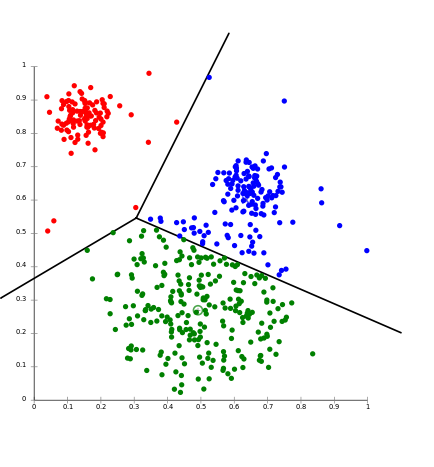
\includegraphics[width=0.45\textwidth, trim=0 30 20 20, clip]
                    {Images/KMeans.png}
    \caption{A visual representation\protect\footnotemark\xspace of the result of \emph{k-means} applied to two-dimensional observations for $k=3$ cluster centers.}
    \label{}
\end{wrapfigure}

\footnotetext{\emph{``KMeans-Gaussian-data"} by Chire - Own work. Licensed under Creative Commons Attribution-Share Alike 3.0 via Wikimedia Commons.}

The vector quantization is based on a \emph{bag-of-words model} to generate the feature vector of each image. First, \emph{k-means} clustering is applied to the extracted \emph{SIFT} descriptors. \\

\emph{K-means} clustering is an algorithm original from signal processing and proposed by Stuart Lloyd in 1982 in its standard version as a technique for \emph{pulse-code modulation} in \cite{Lloyd_1982_LSQ}. It aims to partition \emph{n} observations into \emph{k} clusters in which each observation belongs to the cluster with the nearest mean, serving as a prototype of the cluster. To achieve this, it starts selecting \emph{k} random observations and setting them as cluster centers. Then, it assigns each observation to the closest cluster center and updates the cluster centers by computing the mean of the assigned observations. It repeats the same process till convergence. \\

Therefore, the \emph{SIFT} descriptors are partitioned into \emph{k} clusters, generating \emph{k} clusters centers, which work as \emph{codewords} in the \emph{bag-of-words model}. Finally, each image is assigned a histogram of the \emph{codewords}, which will work as feature vectors in the \emph{SVMs}, by counting the number of \emph{SIFT} descriptors of that image that are ``represented'' by each \emph{codeword}. \\

The \emph{MATLAB} code where this step is implemented and commented at a low-level can be found in the file \texttt{quantizeVectors.m}.

%%%%%%%%%%%
\newpage
\subsubsection{Support Vector Machines (SVMs) for properties recognition}

Once every sample image has its own feature vectors associated, resulting from the vector quantization of the previous step, it is time to train a classifier using them along with the manual markup of properties, which will be the class labels that the classifier will produce. For this purpose, \emph{Support Vector Machines} (\emph{SMVs}) have been used. \\

\begin{wrapfigure}{L}{0pt}
    \centering
    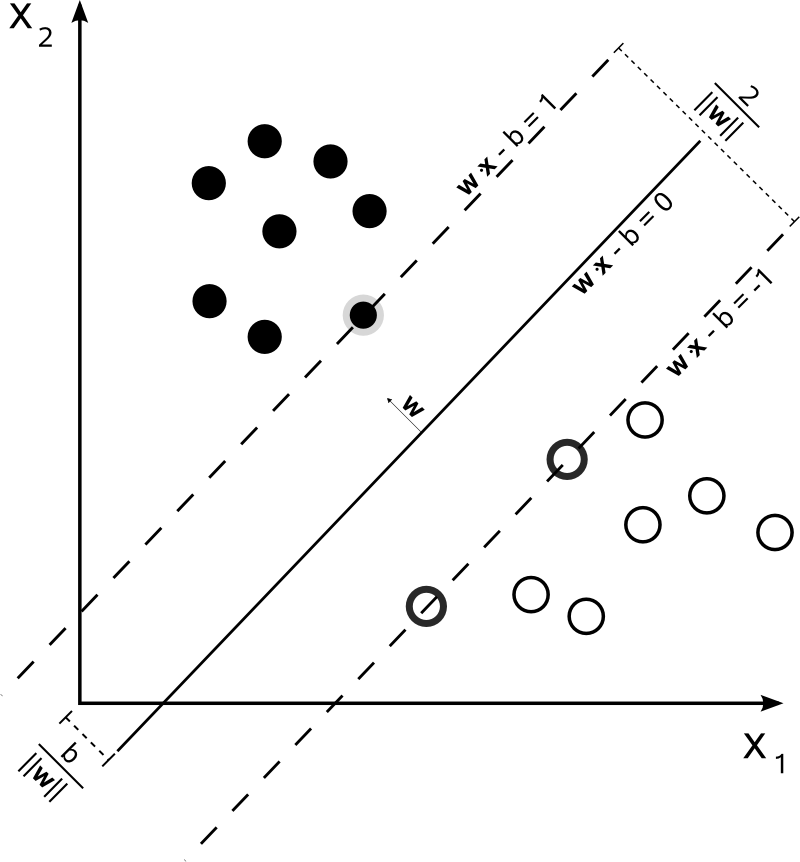
\includegraphics[width=0.4\textwidth, trim=0 0 0 0, clip]
                    {Images/SVMs.png}
    \caption{A visual representation\protect\footnotemark\xspace of the result of the model obtained by a \emph{SVM} algorithm to two-dimensional feature vectors.}
    \label{}
\end{wrapfigure}

\footnotetext{\emph{``Svm max sep hyperplane with margin"} by Cyc - Own work. Licensed under Public domain via Wikimedia Commons.}

\emph{SVMs}, invented by Vladimir Vapnik and published for the first time in \cite{Vapnik_1995_SVMs}, are supervised learning models that work as binary linear classifiers. Given a set of training examples with their respective binary class labels, an \emph{SVM} training algorithm builds a model that assigns, i.e. classifies, new examples into one of the two categories. The built model will define a ($k-1$)-dimensional hyperplane (where \emph{k} is the number of clusters used in the previous step) that will represent the largest separation between the two classes. \\

In our case, one \emph{SVM} is trained for each possible combination of properties and scales that exist in, at least, one of the images of the dataset. In other words, one of the \emph{SVMs} will be used to tell apart material images that present the touch property \emph{bumpy} at \emph{medium} scale, and a different one will decide if a sample is \emph{bumpy} at \emph{coarse} scale, or \emph{extended-organized} at \emph{fine} scale, etc. In the same way, if no image has been manually classified as \emph{feathery} at \emph{fine} scale, no \emph{SVM} will be trained for that property, because of the lack of positive samples. Therefore, the resulting \emph{SVMs}, individually, will only be able to tell if a sample image presents the property at a specific scale or not, since they are binary classifiers. \\

The \emph{MATLAB} code where this step is implemented and commented at a low-level can be found in the file \texttt{svm.m}.


%%%%%%%%%%%%%%%%%%%%%%
\subsection{From properties to materials}

After the properties have been inferred from the material images, a binary feature vector can be built from them for each image considering all the \emph{property-scale} combinations and assigning a 1 if the image has that property or a 0 otherwise.

%%%%%%%%%%%
\subsubsection{Support Vector Machines (SVMs) for material recognition}

The feature vectors combined with the real material labels, allow us to train new \emph{SVMs} for the task of classifying materials from the properties. Unfortunately, the \emph{SVM} model is only suitable for binary classification, i.e., if an image contains a material or not, which is not enough for multi-class classification problem like this. \\

To solve this problem, \emph{Machine Learning} theorists have come up with different strategies. One of them, and the one we use, is \emph{One Vs. All} (\emph{OvA}, a.k.a. \emph{One Vs. Rest} or \emph{OvR}), which consists on training a binary classifier por each class and, when classifying a new sample, applying all of them individually over the sample and considering as result the class of the classifier that gets the highest confidence in the classification. So, for example, if our problem considered three possible materials: \emph{marble}, \emph{brick} and \emph{leather}, and the results of their respective \emph{SVMs} were 3.52, 6.07 and -1.89, the \emph{OvA} would determine that the correct class is \emph{brick}. \\

The \emph{MATLAB} code where this step is implemented and commented at a low-level can be found in the file \texttt{svmOneVsAll.m}.


%%%%%%%%%%%
\subsubsection{Naive Bayes classifier for material recognition}

The properties feature vectors can also be used to fed a different kind of classifier, in this case, more suitable for multi-class classification, as is a \emph{Naive Bayes} classifier. \\

\emph{Naive Bayes} classifiers are another kind of supervised learning models which, unlike \emph{SVMs}, work as probabilistic classifiers instead of linear ones. They are based on the application of the \emph{Bayes' theorem} with strong, i.e. naive, independence assumptions between the features. In other words, it is assummed that the features are independent with respect to each other given the class. \\ 

With all the information computed in the previous steps about the images, a \emph{Naive Bayes} classifier can be trained for material recognition. The \emph{MATLAB} code where this step is implemented and commented at a low-level can be found in the file \texttt{naiveBayes.m}.



%!TEX root = final_report.tex

\section{Approach motivation} \label{sec:approach}

The novelty of the approach strives in the intermediate step of obtaining the material properties in the process of recognition. In other words, instead of trying to infer the class directly from the image descriptors, the properties of the materials are obtained first, and from them, the class of the material. Therefore, its effectiveness depends on the following:

\begin{itemize}
    \item The image feature descriptors, along with the quantization process, are powerful enough to capture precisely the subtleties that determine if a material image presents certain property at a specific scale.
    \item The vocabulary of properties and scales is sufficiently wide and varied to allow a clear distinction between materials. 
\end{itemize}

The ability to choose the most suitable techniques to address this issues will determine the accuracy of the approach.

\subsection{Advantages}

Thanks to the intermediate classification step, the approach presents several clear advantages:

\begin{itemize} 
    \item In case of absolute lack of samples of one class, the approach would, at least, be able to compute its properties if they are present in other samples of the dataset.
    \item A classification of an image with only one training sample of that same material would be possible with relative robustness, again, if its properties are present in other samples.
\end{itemize}   

\subsection{Drawbacks}

Also, some drawbacks are inherent to the use of more steps in the classification process:

\begin{itemize}
    \item The recognition of material properties is based on a supervised learning that requires a costly manual markup of the properties. Unfortunately, the more powerful, varied and precise the vocabulary, the more costly the process of marking the images.
    \item The computational cost of the algorithm increases because of the double recognition problem, first properties, then materials.
\end{itemize}

%!TEX root = final_report.tex

\section{Engineering}

\subsection{Tools}
The main tool used while completing this project has been \emph{MATLAB}. Its  powerful built-in functions and routines for vector and matrix manipulation, along with its wide popularity in academia and, in particular, among the image processing scientists, made it really suitable for the purpose. All the code has been written in \emph{MATLAB} programming language and the debugger that comes with its \emph{IDE} has been widely used to test and polish it. \\

The text editor used to write all the code has been \emph{Sublime Text 2}, because of its flexibility, \emph{MATLAB} syntax highlight and features like multiple cursors or quick selection of the same word, which make the coding task much easier and smooth. \\

This report has been generated using \LaTeX. The main reason to choose it over a \emph{WYSIWYG} editor are the look and feel of the result and its flexibility in many aspects, like the definition of reusable functions or the availability of packages for almost any imaginable task. 


\subsection{Libraries}
\emph{VLFeat} has been the main library for this project. Its functions for \emph{SIFT}, \emph{k-means} and \emph{SVMs} have been really helpful for the implementation. For a complete reference about the library, \cite{Vedaldi_2010_VLFEAT} should be checked. 


\subsection{Maintenance}
Every part of this project has been included in the version-control system \emph{Git} since the beginning, and uploaded frequently to \emph{Github}\footnote{\url{https://github.com/josruice/CS499}}, a website where the code is publicly available. \\

Besides, \emph{MATLAB} code has been written taking into account one of the most important styleguides of the language \cite{Johnson_2002_MPS}, to produce code cleaner and easier to read and understand. Also, comments have been included to emphasize even more the later point. 


% \subsection{Other technical details}


%!TEX root = final_report.tex

\section{Results} \label{sec:results}

%%%%%%%%%%%%%%%%%
\subsection{Parameter tuning}

Given that several steps of the algorithm produce slightly different outputs depending on some predefined parameters, it is natural to have an interest to find the combination of parameter values that gives the best results. \\

In order to achieve that, the following parameters were considered:

\begin{itemize}
    \item Maximum number of \emph{SIFT} descriptors per sample image and, related to it, density of \emph{SIFT} while computing them. If the amount of descriptors exceeded the maximum allowed, they were randomly sampled. Its default value was non-dense \emph{SIFT} without maximum amount of descriptors limitation. The results are shown in figures~\ref{fig:descriptorsTestedPred} and~\ref{fig:descriptorsTestedReal}.
    \item \emph{k} parameter in \emph{k-means}, i.e. number of clusters, with a default value of 300. Its results can be seen in figures~\ref{fig:numberOfClustersTestedPred} and~\ref{fig:numberOfClustersTestedReal}.
    \item $\lambda$ value in \emph{SVMs}, a regularization parameter directly related with the number of iterations performed while computing the best separation hyperplane. Its default value was $10^{-5}$, and the results are represented by figures~\ref{fig:lambdaTestedPred} and~\ref{fig:lambdaTestedReal}.
\end{itemize}

The testing procedure consisted on applying \emph{Cross-Validation} to the dataset, using as test samples a set of 18 images, one per material class, each time. With respect to \emph{Cross-Validation}, it is a widely used model validation technique that allows to measure how the results will generalize to an independent dataset. \\

As can be seen, the models trained using as feature vectors the material properties from the markup get a really good accuracy, around 80\%, almost invariably. This invariability makes sense, specially in the case of the parameter tuning for the number of clusters and the \emph{SIFT} descriptors, since the model are not affected by those. \\

On the other side, the models trained with predicted feature vectors, obtain accuracies around 30\% - 40\% in all cases. When tested independently, the best value of each parameter is  dense \emph{SIFT} (\emph{PHOW}) with a maximum of 1000 descriptors per image, 800 clusters for \emph{k-means} and a \emph{SVMs} $\lambda=0.01$. Nevertheless, when tested as a whole, the best accuracy was obtained by a different, although close, set of parameters, as will be seen.

\plotgnu{../../Figures/descriptorsTestedPred.pdf}
{Graph showing the relation between the material recognition accuracy and the maximum number of \emph{SIFT} descriptors per image, using 300 clusters and \emph{SVMs} $\lambda=10^{-5}$. All these results were obtained using predicted data, i.e. the predicted material properties. In the case of the x-label \emph{SIFT}, no maximum was forced.}
{fig:descriptorsTestedPred}

\plotgnu{../../Figures/descriptorsTestedReal.pdf}
{Graph showing the relation between the material recognition accuracy and the maximum number of \emph{SIFT} descriptors per image, using 300 clusters and \emph{SVMs} $\lambda=10^{-5}$. All these results were obtained using real data, i.e. the material properties from the manual markup. In the case of the x-label \emph{SIFT}, no maximum was forced.}
{fig:descriptorsTestedReal}

\plotgnu{../../Figures/lambdaTestedPred.pdf}
{Graph showing the relation between the material recognition accuracy and the value of \emph{SVMs} $\lambda$, using 300 clusters and non-dense \emph{SIFT} without maximum descriptors limitation. All these results were obtained using predicted data, i.e. the predicted material properties.}
{fig:lambdaTestedPred}

\plotgnu{../../Figures/lambdaTestedReal.pdf}
{Graph showing the relation between the material recognition accuracy and the value of \emph{SVMs} $\lambda$, using 300 clusters and non-dense \emph{SIFT} without maximum descriptors limitation. All these results were obtained using real data, i.e. the material properties from the manual markup.}
{fig:lambdaTestedReal}

\plotgnu{../../Figures/numberOfClustersTestedPred.pdf}
{Graph showing the relation between the material recognition accuracy and the number of clusters in \emph{k-means}, using \emph{SVMs} $\lambda=10^{-5}$ and non-dense \emph{SIFT} without maximum descriptors limitation. All these results were obtained using predicted data, i.e. the predicted material properties.}
{fig:numberOfClustersTestedPred}

\plotgnu{../../Figures/numberOfClustersTestedReal.pdf}
{Graph showing the relation between the material recognition accuracy and the number of clusters in \emph{k-means}, using \emph{SVMs} $\lambda=10^{-5}$ and non-dense \emph{SIFT} without maximum descriptors limitation. All these results were obtained using real data, i.e. the material properties from the manual markup.}
{fig:numberOfClustersTestedReal}


%%%%%%%%%%%%%%%%%
\subsection{Properties recognition accuracy}

As previously said, one of the most important parts of the algorithm is its ability to correctly identify the properties present on the material images. To measure this, the following three metrics have been considered:

\begin{itemize}
    \item \textbf{Global accuracy}: Percentage of classifications where the algorithm correctly identifies that a property is present or that is not present. In other words, true positives plus true negatives, all divided by the total number of samples.
    \item \textbf{Precision}: Percentage of classifications where the algorithm correctly identifies that a property is present over the total number of times it identifies (correctly or uncorrectly) that same property is present, i.e., true positives divided by true positives plus false positives.
    \item \textbf{Recall}: Percentage of classifications where the algorithm correctly identifies that a property is present over the total number of samples that actually present that property. Technically, true positives divided by true positives plus true negatives.
\end{itemize}

The results have been obtained using \emph{Cross-validation} with 12 partitions, guaranteeing that exactly one image of each class was present in every test set. The bar charts for the two first iterations have been plotted, with two versions for every previous metrics: one sorted by material property name (x-axis) and another sorted by the metric value itself (y-axis). The bar charts for the first partition can be seen in the figures~\ref{fig:globalAccuracy3}, ~\ref{fig:globalAccuracySorted3}, ~\ref{fig:precision3}, ~\ref{fig:precisionSorted3}, ~\ref{fig:recall3} and ~\ref{fig:recallSorted3}, while the ones for the second partition are represented in the figures~\ref{fig:globalAccuracy4}, ~\ref{fig:globalAccuracySorted4}, ~\ref{fig:precision4}, ~\ref{fig:precisionSorted4}, ~\ref{fig:recall4} and ~\ref{fig:recallSorted4}. \\

A careful look at the results, reveals that, although the global accuracy seems pretty high for most properties, there is a great room for improvement, as the precision and recall show. Furthermore, in the case of the global accurary, a random classifiers would yield a value approximate to 50\%, which is close, even from the upper part, to the performance obtained in some properties. \\

It can be seen how some properties, like a \emph{flat} shape at \emph{fine} scale, or a \emph{extended disorganized} shape at \emph{medium} scale are hard to recognize for the current set up. On the other side, several touch properties are well recognized at different scales, achieving even a 100\% accuracy. \\

The conclusion that can be extracted from these results is that while \emph{SIFT} descriptors plus vector quantization technique is able to capture enough details for the touch properties, there is still room for improvement in the recognition of shapes.

\plotmatlabbarchart{../../Figures/globalAccuracy3.pdf}
{Bar chart showing the global accuracy in the detection of a property or the lack of it, sorted by \emph{scale-property}. The test set was composed of the first image of each material class, while the rest of the images were part of the training set. Measurements obtained using dense \emph{SIFT} (\emph{PHOW}) limited to a maximum of 2000 descriptors per image, with 600 clusters and \emph{SVM} $\lambda=10^{-3}$.}
{fig:globalAccuracy3}

\plotmatlabbarchart{../../Figures/globalAccuracySorted3.pdf}
{Bar chart showing the global accuracy in the detection of a property or the lack of it, sorted by the accuracy itself. The test set was composed of the first image of each material class, while the rest of the images were part of the training set. Measurements obtained using dense \emph{SIFT} (\emph{PHOW}) limited to a maximum of 2000 descriptors per image, with 600 clusters and \emph{SVM} $\lambda=10^{-3}$.}
{fig:globalAccuracySorted3}

\plotmatlabbarchart{../../Figures/precision3.pdf}
{Bar chart showing the \emph{precision} in the detection of a property, i.e. the number of true positives over the total number of image samples that has been classified as having the property, sorted by \emph{scale-property}. The test set was composed of the first image of each material class, while the rest of the images were part of the training set. Measurements obtained using dense \emph{SIFT} (\emph{PHOW}) limited to a maximum of 2000 descriptors per image, with 600 clusters and \emph{SVM} $\lambda=10^{-3}$.}
{fig:precision3}

\plotmatlabbarchart{../../Figures/precisionSorted3.pdf}
{Bar chart showing the \emph{precision} in the detection of a property, i.e. the number of true positives over the total number of image samples that has been classified as having the property, sorted by the \emph{precision} itself. The test set was composed of the first image of each material class, while the rest of the images were part of the training set. Measurements obtained using dense \emph{SIFT} (\emph{PHOW}) limited to a maximum of 2000 descriptors per image, with 600 clusters and \emph{SVM} $\lambda=10^{-3}$.}
{fig:precisionSorted3}

\plotmatlabbarchart{../../Figures/recall3.pdf}
{Bar chart showing the \emph{recall} in the detection of a property, i.e. the number of true positives over the total number of image samples with the property, sorted by \emph{scale-property}. The test set was composed of the first image of each material class, while the rest of the images were part of the training set. Measurements obtained using dense \emph{SIFT} (\emph{PHOW}) limited to a maximum of 2000 descriptors per image, with 600 clusters and \emph{SVM} $\lambda=10^{-3}$.}
{fig:recall3}

\plotmatlabbarchart{../../Figures/recallSorted3.pdf}
{Bar chart showing the \emph{recall} in the detection of a property, i.e. the number of true positives over the total number of image samples with the property, sorted by the \emph{recall} itself. The test set was composed of the first image of each material class, while the rest of the images were part of the training set. Measurements obtained using dense \emph{SIFT} (\emph{PHOW}) limited to a maximum of 2000 descriptors per image, with 600 clusters and \emph{SVM} $\lambda=10^{-3}$.}
{fig:recallSorted3}


\plotmatlabbarchart{../../Figures/globalAccuracy4.pdf}
{Bar chart showing the global accuracy in the detection of a property or the lack of ifig:t, sorted by \emph{scale-property}. The test set was composed of the second image of each material class, while the rest of the images were part of the training set. Measurements obtained using dense \emph{SIFT} (\emph{PHOW}) limited to a maximum of 2000 descriptors per image, with 600 clusters and \emph{SVM} $\lambda=10^{-3}$.}
{fig:globalAccuracy4}

\plotmatlabbarchart{../../Figures/globalAccuracySorted4.pdf}
{Bar chart showing the global accuracy in the detection of a property or the lack of ifig:t, sorted by the accuracy itself. The test set was composed of the second image of each material class, while the rest of the images were part of the training set. Measurements obtained using dense \emph{SIFT} (\emph{PHOW}) limited to a maximum of 2000 descriptors per image, with 600 clusters and \emph{SVM} $\lambda=10^{-3}$.}
{fig:globalAccuracySorted4}

\plotmatlabbarchart{../../Figures/precision4.pdf}
{Bar chart showing the \emph{precision} in the detection of a property, i.e. the number of true positives over the total number of image samples that has been classified as having the property, sorted by \emph{scale-property}. The test set was composed of the second image of each material class, while the rest of the images were part of the training set. Measurements obtained using dense \emph{SIFT} (\emph{PHOW}) limited to a maximum of 2000 descriptors per image, with 600 clusters and \emph{SVM} $\lambda=10^{-3}$.}
{fig:precision4}

\plotmatlabbarchart{../../Figures/precisionSorted4.pdf}
{Bar chart showing the \emph{precision} in the detection of a property, i.e. the number of true positives over the total number of image samples that has been classified as having the property, sorted by the \emph{precision} itself. The test set was composed of the second image of each material class, while the rest of the images were part of the training set. Measurements obtained using dense \emph{SIFT} (\emph{PHOW}) limited to a maximum of 2000 descriptors per image, with 600 clusters and \emph{SVM} $\lambda=10^{-3}$.}
{fig:precisionSorted4}

\plotmatlabbarchart{../../Figures/recall4.pdf}
{Bar chart showing the \emph{recall} in the detection of a property, i.e. the number of true positives over the total number of image samples with the property, sorted by \emph{scale-property}. The test set was composed of the second image of each material class, while the rest of the images were part of the training set. Measurements obtained using dense \emph{SIFT} (\emph{PHOW}) limited to a maximum of 2000 descriptors per image, with 600 clusters and \emph{SVM} $\lambda=10^{-3}$.}
{fig:recall4}

\plotmatlabbarchart{../../Figures/recallSorted4.pdf}
{Bar chart showing the \emph{recall} in the detection of a property, i.e. the number of true positives over the total number of image samples with the property, sorted by the \emph{recall} itself. The test set was composed of the second image of each material class, while the rest of the images were part of the training set. Measurements obtained using dense \emph{SIFT} (\emph{PHOW}) limited to a maximum of 2000 descriptors per image, with 600 clusters and \emph{SVM} $\lambda=10^{-3}$.}
{fig:recallSorted4}



%%%%%%%%%%%%%%%%%
\subsection{Confusion matrices}

The last part of the algorithm consists on recognizing the material using the properties extracted from each image. There is no need to highlight the great importance of this step, since this is the main purpose for the whole algorithm. \\

A widely used method to measure the performance of multi-class classification algorithms are the \emph{confusion matrices}. This mathematical tool represents the results as a matrix with the same number of rows and columns as possible classes, and in which the cell in row $i$, column $j$ represents the percentage of times an image of $i^{th}$ class has been classified as an image of $j^{th}$ class. In this situation, the best classifiers will be those that achieve results closer to 1 (or 100\%) in the main diagonal of the matrix, being the ideal a perfect diagonal matrix with all 1. \\

The \emph{confusion matrices} represented in figures~\ref{fig:svmPredPred}, ~\ref{fig:svmPredReal}, ~\ref{fig:svmRealPred}, ~\ref{fig:svmRealReal}, ~\ref{fig:nbPredPred}, ~\ref{fig:nbPredReal}, ~\ref{fig:nbRealPred}, ~\ref{fig:nbRealReal}, show the results for \emph{SVMs} and \emph{Naive Bayes} for all the possible combinations of training and testing using data predicted by the algorithm or data extracted from the manual markup, assummed to be real data. \\

As before, a \emph{Cross-validation} process with 12 partitions have been used, guaranteeing that exactly one image of each class was present in every test set. In this case, the averaged sum of the confusion matrices of every iteration is represented in each image. \\

As can be seen, the most striking fact is that the classifiers tested with feature vectors extracted from the manual markup are able to classify with much higher accuracy, in some cases, almost as twice. The use of this kind of data for the testing part allow us to see the theoretical limitation of the model, since it represents the performance assumming perfect results in the process of recognizing the material properties. The fact that the achieved accuracy with this data is above 80\% is a good sign of the ability of the vocabulary to capture the difference between material classes. \\

The \emph{confusion matrices} also give us insights about what classes are close to each other in terms of properties, taking into account the current vocabulary. For example, a fair amount of \emph{concrete} samples are classified as \emph{stucco}, and the other way around. Also, it can be extracted which classes lose more information in the property recognition process, since they get almost no correct classifications when testing the predicted properties. Examples of this are \emph{denim} and \emph{knitguernsey}. \\

\plotmatlabconfusion{../../Figures/nbPredPred.png}
{Heat map representing the confusion matrix of the material recognition process using \emph{Naive Bayes} trained with predicted data, i.e., properties estimated algorithmically, and tested also with predicted data. The results are the average of a \emph{cross-validation} process of 12 partitions, where the test set had at least one sample of each class. The parameters used are dense \emph{SIFT} (\emph{PHOW}) limited to a maximum of 2000 descriptors per image, with 600 clusters and \emph{SVM} $\lambda=10^{-3}$. The average precision obtained is 45.37 \%, with 98 out of 216 samples correctly classified.}
{fig:nbPredPred}

\plotmatlabconfusion{../../Figures/nbPredReal.png}
{Heat map representing the confusion matrix of the material recognition process using \emph{Naive Bayes} trained with predicted data, i.e., properties estimated algorithmically, and tested with real data, i.e., properties extracted from the manual markup. The results are the average of a \emph{cross-validation} process of 12 partitions, where the test set had at least one sample of each class. The parameters used are dense \emph{SIFT} (\emph{PHOW}) limited to a maximum of 2000 descriptors per image, with 600 clusters and \emph{SVM} $\lambda=10^{-3}$. The average precision obtained is 80.56 \%, with 174 out of 216 samples correctly classified.}
{fig:nbPredReal}

\plotmatlabconfusion{../../Figures/nbRealPred.png}
{Heat map representing the confusion matrix of the material recognition process using \emph{Naive Bayes} trained with real data, i.e., properties extracted from the manual markup, and tested with predicted data, i.e., properties estimated algorithmically. The results are the average of a \emph{cross-validation} process of 12 partitions, where the test set had at least one sample of each class. The parameters used are dense \emph{SIFT} (\emph{PHOW}) limited to a maximum of 2000 descriptors per image, with 600 clusters and \emph{SVM} $\lambda=10^{-3}$. The average precision obtained is 46.30 \%, with 100 out of 216 samples correctly classified.}
{fig:nbRealPred}

\plotmatlabconfusion{../../Figures/nbRealReal.png}
{Heat map representing the confusion matrix of the material recognition process using \emph{Naive Bayes} trained with real data, i.e., properties extracted from the manual markup, and tested also with predicted data. The results are the average of a \emph{cross-validation} process of 12 partitions, where the test set had at least one sample of each class. The parameters used are dense \emph{SIFT} (\emph{PHOW}) limited to a maximum of 2000 descriptors per image, with 600 clusters and \emph{SVM} $\lambda=10^{-3}$. The average precision obtained is 79.63 \%, with 172 out of 216 samples correctly classified.}
{fig:nbRealReal}


\plotmatlabconfusion{../../Figures/svmPredPred.png}
{Heat map representing the confusion matrix of the material recognition process using \emph{SVMs} trained with predicted data, i.e., properties estimated algorithmically, and tested also with predicted data. The results are the average of a \emph{cross-validation} process of 12 partitions, where the test set had at least one sample of each class. The parameters used are dense \emph{SIFT} (\emph{PHOW}) limited to a maximum of 2000 descriptors per image, with 600 clusters and \emph{SVM} $\lambda=10^{-3}$. The average precision obtained is 44.44 \%, with 96 out of 216 samples correctly classified.}
{fig:svmPredPred}

\plotmatlabconfusion{../../Figures/svmPredReal.png}
{Heat map representing the confusion matrix of the material recognition process using \emph{SVMs} trained with predicted data, i.e., properties estimated algorithmically, and tested with real data, i.e., properties extracted from the manual markup. The results are the average of a \emph{cross-validation} process of 12 partitions, where the test set had at least one sample of each class. The parameters used are dense \emph{SIFT} (\emph{PHOW}) limited to a maximum of 2000 descriptors per image, with 600 clusters and \emph{SVM} $\lambda=10^{-3}$. The average precision obtained is 81.02 \%, with 175 out of 216 samples correctly classified.}
{fig:svmPredReal}

\plotmatlabconfusion{../../Figures/svmRealPred.png}
{Heat map representing the confusion matrix of the material recognition process using \emph{SVMs} trained with real data, i.e., properties extracted from the manual markup, and tested with predicted data, i.e., properties estimated algorithmically. The results are the average of a \emph{cross-validation} process of 12 partitions, where the test set had at least one sample of each class. The parameters used are dense \emph{SIFT} (\emph{PHOW}) limited to a maximum of 2000 descriptors per image, with 600 clusters and \emph{SVM} $\lambda=10^{-3}$. The average precision obtained is 44.44 \%, with 96 out of 216 samples correctly classified.}
{fig:svmRealPred}

\plotmatlabconfusion{../../Figures/svmRealReal.png}
{Heat map representing the confusion matrix of the material recognition process using \emph{SVMs} trained with real data, i.e., properties extracted from the manual markup, and tested also with predicted data. The results are the average of a \emph{cross-validation} process of 12 partitions, where the test set had at least one sample of each class. The parameters used are dense \emph{SIFT} (\emph{PHOW}) limited to a maximum of 2000 descriptors per image, with 600 clusters and \emph{SVM} $\lambda=10^{-3}$. The average precision obtained is 82.41 \%, with 178 out of 216 samples correctly classified.}
{fig:svmRealReal}



%%%%%%%%%%%%%%%%%
\subsection{Material recognition accuracy}

The randomness inherent to some of the steps of techniques such as \emph{k-means} and \emph{SVMs} yield different results even when using the same parameters. Taking this into account, the best accuracy was obtained in an execution of the algorithm using the same set up as the graphs and bar charts shown above, i.e., \emph{SIFT} (\emph{PHOW}) limited to a maximum of 2000 descriptors per image, with 600 clusters and \emph{SVM} $\lambda=10^{-3}$. The number of correctly classifier samples were the following:

\begin{itemize}
    \item 95 out of 216 (43.98 \%) in \emph{NB} trained with predicted data and tested with predicted data.
    \item 172 out of 216 (79.63 \%) in \emph{NB} trained with predicted data and tested with real data.
    \item 93 out of 216 (43.06 \%) in \emph{NB} trained with real data and tested with predicted data.
    \item 172 out of 216 (79.63 \%) in \emph{NB} trained with real data and tested with real data.
    \item 101 out of 216 (46.76 \%) in \emph{SVMs} trained with predicted data and tested with predicted data.
    \item 178 out of 216 (82.41 \%) in \emph{SVMs} trained with predicted data and tested with real data.
    \item 103 out of 216 (47.69 \%) in \emph{SVMs} trained with real data and tested with predicted data.
    \item 178 out of 216 (82.41 \%) in \emph{SVMs} trained with real data and tested with real data.
\end{itemize}

As can be seen, the trend with respect to the testing data is the same as in previous executions, and the results are in the same range, although some points above. \\

The result of this execution can be compared in terms of accuracy with the ones shown in \cite{Liao_2013_CVPR}, where the most accurate method, the one presented in the paper, gets a modest 43.5 \%. Therefore, the approach introduced in this work beats all the other approaches to the problem using this dataset. 


%!TEX root = final_report.tex

\section{Conclusions and future work} \label{sec:conclusions}

Material recognition using \emph{Computer Vision} is still an open problem in the industry. Many different approaches have been tried to solve it, being \emph{Deep Learning} the one that, nowadays, is giving the most promising results. \\

Even though, it is still worth it to try different, new approaches. In this work, we have covered a solution based on classic \emph{Machine Learning} techniques, such as \emph{SVMs}, \emph{k-means} and \emph{Naive Bayes}, along with the powerful and widely used \emph{SIFT} descriptors, but including an innovation in the use of an intermediate step based on a vocabulary of material properties. \\

We have analyzed the hightlights and lowlights of the approach, both from a theoretical and practical point of view, providing results using several metrics for different parts of the algorithm. \\

While the results look promising when using the real material properties to classify materials, further research is required to test the effects of a higher dataset and different feature descriptors methods in terms of accuracy. Even if better results are achieved in harsher conditions, the high cost of the manual markup of properties is still an important drawback of the algorithm. \\

Apart from the material recognition use, it cannot be denied that the information obtained in the intermediate step provides value to the classification process that could be useful even in real life applications. Besides, the theoretical possibility of one sample classification is interesting enough to motivate the continuation of this work.

\bibliography{final_bibliography}
\bibliographystyle{abbrv}

\begin{appendix}
    %!TEX root = final_report.tex

%%%%%%%%
\section{Markup}

% Markup commands.
\newcommand{\imageSize}{0.30}
\newcommand{\dataSize}{0.65}
\newcommand{\spaceSize}{0.02}

\newcommand{\mat}{Birch}
\newcommand{\Number}{01}
\newcommand{\InputImage}[8]{
\begin{figure}[!ht]
    \centering
    \begin{minipage}{\imageSize\textwidth}
        \centering
        \includegraphics[width=\textwidth]{../../Dataset/\mat/\Number.png}
    \end{minipage}
    \hspace{\spaceSize\textwidth}
    \begin{minipage}{\dataSize\textwidth}
        \textbf{\large \mat \xspace \Number}:

        #7
        \begin{itemize}
            \item \Fine: #1, #2.
            \item \Medium: #3, #4.
            \item \Coarse: #5, #6.
        \end{itemize}
        #8
    \end{minipage}
\end{figure}
\FloatBarrier    
}

%%%
\renewcommand{\mat}{Birch}
\subsection{\mat}
Coarse scale is considered the picture itself, while medium scale is a part where the horizontal pattern is not present, and fine scale a little spot in the medium scale.

\renewcommand{\Number}{01}\InputImage{\sfl}{\tco}{\sexdi}{\tsc}{\sexor}{\tsc}
{}{}
\renewcommand{\Number}{02}\InputImage{\sfl}{\tco}{\sfl}{\tco}{\sexdi}{\tsc}
{}{}
\renewcommand{\Number}{03}\InputImage{\sfl}{\tco}{\sexor}{\tsc}{\sexor}{\tsc}
{}{}
\renewcommand{\Number}{04}\InputImage{\sfl}{\tco}{\sexor}{\tsc}{\sro}{\tco}
{Watermark and big crack.}{}
\renewcommand{\Number}{05}\InputImage{\sfl}{\tco}{\sfl}{\tco}{\sexor}{\tsc}
{}{Considering for the medium scale the part without horizontal lines.}
\renewcommand{\Number}{06}\InputImage{\sfl}{\tco}{\sexor}{\tsc}{\sexor}{\tsc}
{}{}
\renewcommand{\Number}{07}\InputImage{\sfl}{\tco}{\sexor}{\tco}{\sexor}{\tco}
{}{}
\renewcommand{\Number}{08}\InputImage{\sfl}{\tco}{\sexor}{\tsc}{\sexor}{\tsc}
{Watermark.}{}
\renewcommand{\Number}{09}\InputImage{\sfl}{\tco}{\sexor}{\tsc}{\sexdi}{\tsc}
{}{}
\renewcommand{\Number}{10}\InputImage{\sfl}{\tco}{\sexor}{\tsc}{\sexor}{\tsc}
{}{}
\renewcommand{\Number}{11}\InputImage{\sfl}{\tco}{\sexor}{\tsc}{\sro}{\tsc}
{Big crack.}{}
\renewcommand{\Number}{12}\InputImage{\sfl}{\tco}{\sexor}{\tsc}{\sexor}{\tsc}
{}{}

%%%
\clearpage
\renewcommand{\mat}{Brick}
\subsection{\mat}

\renewcommand{\Number}{01}\InputImage{\sfl}{\tco}{\sexor}{\tco}{\sexor}{\tco}
{}{}
\renewcommand{\Number}{02}\InputImage{\sfl}{\tsc}{\sexor}{\tco}{\sexor}{\tco}
{}{Considering as fine scale the mortar.}
\renewcommand{\Number}{03}\InputImage{\sfl}{\tsc}{\sfl}{\tco}{\sexor}{\tsc}
{}{Considering as fine scale the mortar.}
\renewcommand{\Number}{04}\InputImage{\sfl}{\tco}{\sexor}{\tco}{\sexor}{\tco}
{}{}
\renewcommand{\Number}{05}\InputImage{\sfl}{\tco}{\sexor}{\tco}{\sexor}{\tco}
{}{Might also be considered bumpy at coarse and medium scale?}
\renewcommand{\Number}{06}\InputImage{\sfl}{\tco}{\sexor}{\tsm}{\sexor}{\tsm}
{Graffiti.}{Considering as fine scale the mortar.}
\renewcommand{\Number}{07}\InputImage{\sfl}{\tco}{\sexor}{\tco}{\sexor}{\tco}
{}{}
\renewcommand{\Number}{08}\InputImage{\sfl}{\tco}{\sexor}{\tbu}{\sexor}{\tbu}
{}{}
\renewcommand{\Number}{09}\InputImage{\sfl}{\tco}{\sexor}{\tco}{\sexor}{\tco}
{}{}
\renewcommand{\Number}{10}\InputImage{\sfl}{\tsc}{\sexor}{\tco}{\sexor}{\tco}
{}{Considering as fine scale the mortar.}
\renewcommand{\Number}{11}\InputImage{\sexor}{\tco}{\sexor}{\tco}{\sexor}{\tco}
{}{}
\renewcommand{\Number}{12}\InputImage{\sfl}{\tsm}{\sexor}{\tsm}{\sexor}{\tbu}
{}{}

%%%
\clearpage
\renewcommand{\mat}{Concrete}
\subsection{\mat}

\renewcommand{\Number}{01}\InputImage{\sfl}{\tco}{\sfl}{\tco}{\sfl}{\tco}
{}{}
\renewcommand{\Number}{02}\InputImage{\sfl}{\tco}{\sfl}{\tco}{\sexdi}{\tco}
{}{}
\renewcommand{\Number}{03}\InputImage{\sfl}{\tco}{\sfl}{\tco}{\sexdi}{\tbu}
{}{}
\renewcommand{\Number}{04}\InputImage{\sfl}{\tsc}{\sfl}{\tsc}{\sfl}{\tsc}
{}{}
\renewcommand{\Number}{05}\InputImage{\sfl}{\tco}{\sfl}{\tco}{\sexor}{\tco}
{}{}
\renewcommand{\Number}{06}\InputImage{\sfl}{\tco}{\sfl}{\tco}{\sexor}{\tco}
{}{Considering that the almost straight break is organized.}
\renewcommand{\Number}{07}\InputImage{\sfl}{\tco}{\sfl}{\tco}{\sro}{\tsc}
{}{Considering the spots of different colours to determine a round shape.}
\renewcommand{\Number}{08}\InputImage{\sfl}{\tco}{\sfl}{\tco}{\sfl}{\tco}
{}{Considering that the patterns in the middle of the image don't affect the shape.}
\renewcommand{\Number}{09}\InputImage{\sfl}{\tco}{\sfl}{\tco}{\sfl}{\tco}
{}{}
\renewcommand{\Number}{10}\InputImage{\sfl}{\tco}{\sfl}{\tco}{\sexdi}{\tco}
{}{}
\renewcommand{\Number}{11}\InputImage{\sfl}{\tco}{\sfl}{\tsc}{\sfl}{\tsc}
{}{}
\renewcommand{\Number}{12}\InputImage{\sfl}{\tsc}{\sfl}{\tsc}{\sfl}{\tsc}
{}{}

%%%
\clearpage
\renewcommand{\mat}{Corduroy}
\subsection{\mat}

\renewcommand{\Number}{01}\InputImage{\sexor}{\tsm}{\sexor}{\tsm}{\sexor}{\tbu}
{Logo in the right bottom corner.}{}
\renewcommand{\Number}{02}\InputImage{\sfl}{\tve}{\sexor}{\tbu}{\sexdi}{\tbu}
{}{Considering that the perpendicular direction of the lines makes them disorganized.}
\renewcommand{\Number}{03}\InputImage{\sfl}{\tsm}{\sexor}{\tbu}{\sexdi}{\tbu}
{}{}
\renewcommand{\Number}{04}\InputImage{\sfl}{\tsm}{\sexor}{\tbu}{\sexdi}{\tbu}
{}{}
\renewcommand{\Number}{05}\InputImage{\sfl}{\tve}{\sexor}{\tbu}{\sexdi}{\tbu}
{}{}
\renewcommand{\Number}{06}\InputImage{\sfl}{\tve}{\sexor}{\tbu}{\sro}{\tbu}
{}{Considering the buttons as part of the course scale.}
\renewcommand{\Number}{07}\InputImage{\sfl}{\tve}{\sexor}{\tbu}{\sexor}{\tbu}
{}{}
\renewcommand{\Number}{08}\InputImage{\sfl}{\tve}{\sexor}{\tbu}{\sexor}{\tbu}
{Logo in the bottom left corner.}{}
\renewcommand{\Number}{09}\InputImage{\sfl}{\tve}{\sexor}{\tbu}{\sexor}{\tbu}
{}{}
\renewcommand{\Number}{10}\InputImage{\sexor}{\tbu}{\sexor}{\tbu}{\sro}{\tbu}
{}{Considering the figures of the bottom left corner for the coarse scale.}
\renewcommand{\Number}{11}\InputImage{\sfl}{\tve}{\sexor}{\tbu}{\sexor}{\tbu}
{}{}
\renewcommand{\Number}{12}\InputImage{\sexor}{\tbu}{\sexor}{\tbu}{\sro}{\tbu}
{}{Considering the flower for the coarse scale.}

%%%
\clearpage
\renewcommand{\mat}{Denim}
\subsection{\mat}

\renewcommand{\Number}{01}\InputImage{\sexor}{\tsm}{\sexor}{\tsm}{\sexor}{\tsm}
{}{}
\renewcommand{\Number}{02}\InputImage{\sexor}{\tsm}{\sexor}{\tsm}{\sexor}{\tsm}
{}{}
\renewcommand{\Number}{03}\InputImage{\sexor}{\tsm}{\sexor}{\tsm}{\sexdi}{\tbu}
{}{}
\renewcommand{\Number}{04}\InputImage{\sexor}{\tsm}{\sexor}{\tsm}{\sexdi}{\tbu}
{}{}
\renewcommand{\Number}{05}\InputImage{\sexor}{\tsm}{\sexor}{\tsm}{\sexor}{\tsm}
{}{}
\renewcommand{\Number}{06}\InputImage{\sro}{\tsm}{\sro}{\tsm}{\sro}{\tsm}
{}{}
\renewcommand{\Number}{07}\InputImage{\sexor}{\tsm}{\sexor}{\tsm}{\sexdi}{\tsm}
{}{}
\renewcommand{\Number}{08}\InputImage{\sexor}{\tsm}{\sexor}{\tsm}{\sexor}{\tsm}
{Watermark.}{}
\renewcommand{\Number}{09}\InputImage{\sro}{\tsm}{\sro}{\tsm}{\sro}{\tsm}
{}{}
\renewcommand{\Number}{10}\InputImage{\sexor}{\tsm}{\sexor}{\tsm}{\sexdi}{\tbu}
{}{}
\renewcommand{\Number}{11}\InputImage{\sro}{\tsm}{\sro}{\tsm}{\sro}{\tbu}
{}{}
\renewcommand{\Number}{12}\InputImage{\sro}{\tsm}{\sro}{\tsm}{\sro}{\tbu}
{}{}

%%%
\clearpage
\renewcommand{\mat}{Elm}
\subsection{\mat}

\renewcommand{\Number}{01}\InputImage{\sfl}{\tco}{\sexdi}{\tbu}{\sexdi}{\tbu}
{}{Considering the bark to be disorganized.}
\renewcommand{\Number}{02}\InputImage{\sfl}{\tco}{\sro}{\tbu}{\sro}{\tbu}
{}{}
\renewcommand{\Number}{03}\InputImage{\sfl}{\tco}{\sexdi}{\tbu}{\sexdi}{\tbu}
{}{}
\renewcommand{\Number}{04}\InputImage{\sfl}{\tco}{\sexdi}{\tbu}{\sexdi}{\tbu}
{}{}
\renewcommand{\Number}{05}\InputImage{\sfl}{\tco}{\sexdi}{\tbu}{\sexdi}{\tbu}
{}{}
\renewcommand{\Number}{06}\InputImage{\sfl}{\tco}{\sexor}{\tbu}{\sexor}{\tbu}
{}{Considering the bark as organized.}
\renewcommand{\Number}{07}\InputImage{\sfl}{\tco}{\sexdi}{\tbu}{\sexdi}{\tbu}
{}{}
\renewcommand{\Number}{08}\InputImage{\sfl}{\tco}{\sexdi}{\tbu}{\sexdi}{\tbu}
{}{}
\renewcommand{\Number}{09}\InputImage{\sfl}{\tco}{\sexdi}{\tbu}{\sexdi}{\tbu}
{}{}
\renewcommand{\Number}{10}\InputImage{\sfl}{\tco}{\sfl}{\tco}{\sexdi}{\tbu}
{}{}
\renewcommand{\Number}{11}\InputImage{\sfl}{\tco}{\sexdi}{\tbu}{\sexdi}{\tbu}
{Extremely low quality image.}{}
\renewcommand{\Number}{12}\InputImage{\sfl}{\tco}{\sro}{\tbu}{\sro}{\tbu}
{}{}

%%%
\clearpage
\renewcommand{\mat}{Feathers}
\subsection{\mat}

\renewcommand{\Number}{01}\InputImage{\sexor}{\tbu}{\sexor}{\tbu}{\sro}{\tfe}
{Watermark.}{}
\renewcommand{\Number}{02}\InputImage{\sexor}{\tbu}{\sexor}{\tbu}{\sro}{\tfe} 
{}{}
\renewcommand{\Number}{03}\InputImage{\sexor}{\tbu}{\sexor}{\tbu}{\sro}{\tfe} 
{}{}
\renewcommand{\Number}{04}\InputImage{\sexor}{\tbu}{\sexor}{\tbu}{\sexdi}{\tfe}
{}{}
\renewcommand{\Number}{05}\InputImage{\sexor}{\tbu}{\sro}{\tfe}{\sro}{\tfe}
{Watermark.}{}
\renewcommand{\Number}{06}\InputImage{\sfl}{\tsm}{\sro}{\tfe}{\sro}{\tfe}
{}{}
\renewcommand{\Number}{07}\InputImage{\sexor}{\tbu}{\sexdi}{\tfe}{\sexdi}{\tfe}
{}{}
\renewcommand{\Number}{08}\InputImage{\sexor}{\tbu}{\sexor}{\tbu}{\sexdi}{\tfe}
{}{}
\renewcommand{\Number}{09}\InputImage{\sexor}{\tbu}{\sexor}{\tbu}{\sexdi}{\tfe}
{}{}
\renewcommand{\Number}{10}\InputImage{\sfl}{\tsm}{\sro}{\tfe}{\sro}{\tfe}
{}{Considering the wing for the medium scale.}
\renewcommand{\Number}{11}\InputImage{\sexor}{\tbu}{\sexor}{\tfe}{\sexor}{\tfe}
{}{}
\renewcommand{\Number}{12}\InputImage{\sexor}{\tbu}{\sro}{\tfe}{\sro}{\tfe}
{}{}

%%%
\clearpage
\renewcommand{\mat}{Fur}
\subsection{\mat}
Considering that the pattern that follows the fur is, at least, at low scale, organized.

\renewcommand{\Number}{01}\InputImage{\sexor}{\tfu}{\sexor}{\tfu}{\sexdi}{\tfu}
{Watermark.}{}
\renewcommand{\Number}{02}\InputImage{\sexor}{\tfu}{\sexor}{\tfu}{\sexdi}{\tfu}
{}{}
\renewcommand{\Number}{03}\InputImage{\sexor}{\tfu}{\sexor}{\tfu}{\sro}{\tfu}
{}{Considering the spots as elements of round shape.}
\renewcommand{\Number}{04}\InputImage{\sexor}{\tfu}{\sexor}{\tfu}{\sexor}{\tfu}
{}{}
\renewcommand{\Number}{05}\InputImage{\sexor}{\tfu}{\sexor}{\tfu}{\sexdi}{\tfu}
{}{}
\renewcommand{\Number}{06}\InputImage{\sexor}{\tfu}{\sexor}{\tfu}{\sexdi}{\tfu}
{}{}
\renewcommand{\Number}{07}\InputImage{\sexor}{\tfu}{\sexdi}{\tfu}{\sexdi}{\tfu}
{}{}
\renewcommand{\Number}{08}\InputImage{\sexor}{\tfu}{\sexor}{\tfu}{\sexdi}{\tfu}
{}{}
\renewcommand{\Number}{09}\InputImage{\sexor}{\tfu}{\sexdi}{\tfu}{\sexdi}{\tfu}
{}{}
\renewcommand{\Number}{10}\InputImage{\sexor}{\tfu}{\sexor}{\tfu}{\sexdi}{\tfu}
{}{}
\renewcommand{\Number}{11}\InputImage{\sexor}{\tfu}{\sexor}{\tfu}{\sro}{\tfu}
{Same as Fur 03 with different color.}{}
\renewcommand{\Number}{12}\InputImage{\sexor}{\tfu}{\sexor}{\tfu}{\sexdi}{\tfu}
{}{}

%%%
\clearpage
\renewcommand{\mat}{Hair}
\subsection{\mat}
Considering that the touch of hair is smooth at a high scale.

\renewcommand{\Number}{01}\InputImage{\sexor}{\tbu}{\sexor}{\tsm}{\sexdi}{\tsm}
{Watermark.}{}
\renewcommand{\Number}{02}\InputImage{\sexor}{\tbu}{\sexdi}{\tsm}{\sexdi}{\tsm}
{Watermark.}{}
\renewcommand{\Number}{03}\InputImage{\sexor}{\tbu}{\sexor}{\tsm}{\sexdi}{\tsm}
{}{}
\renewcommand{\Number}{04}\InputImage{\sexor}{\tbu}{\sexor}{\tsm}{\sexdi}{\tsm}
{}{}
\renewcommand{\Number}{05}\InputImage{\sexor}{\tbu}{\sexor}{\tsm}{\sexor}{\tsm}
{}{}
\renewcommand{\Number}{06}\InputImage{\sexor}{\tbu}{\sexor}{\tsm}{\sexor}{\tsm}
{}{}
\renewcommand{\Number}{07}\InputImage{\sexor}{\tbu}{\sexor}{\tsm}{\sexdi}{\tsm}
{}{}
\renewcommand{\Number}{08}\InputImage{\sexor}{\tbu}{\sexdi}{\tsm}{\sexdi}{\tsm}
{}{}
\renewcommand{\Number}{09}\InputImage{\sexor}{\tbu}{\sexor}{\tsm}{\sexdi}{\tsm}
{}{}
\renewcommand{\Number}{10}\InputImage{\sexor}{\tbu}{\sexor}{\tsm}{\sexdi}{\tsm}
{Watermark.}{}
\renewcommand{\Number}{11}\InputImage{\sexor}{\tbu}{\sexor}{\tsm}{\sexor}{\tsm}
{}{}
\renewcommand{\Number}{12}\InputImage{\sexor}{\tbu}{\sexor}{\tsm}{\sexdi}{\tsm}
{}{}

%%%
\clearpage
\renewcommand{\mat}{KnitAran}
\subsection{\mat}
Considering that non-linear patterns are disorganized.

\renewcommand{\Number}{01}\InputImage{\sexor}{\tco}{\sexdi}{\tbu}{\sexdi}{\tbu}
{}{}
\renewcommand{\Number}{02}\InputImage{\sexdi}{\tco}{\sexdi}{\tbu}{\sexdi}{\tbu}
{}{}
\renewcommand{\Number}{03}\InputImage{\sexor}{\tco}{\sexdi}{\tbu}{\sexdi}{\tbu}
{}{Considering that the round parts of the pattern are extended disorganized.}
\renewcommand{\Number}{04}\InputImage{\sexor}{\tco}{\sexdi}{\tbu}{\sro}{\tbu}
{}{Considering the buttons at the coarse level.}
\renewcommand{\Number}{05}\InputImage{\sexor}{\tco}{\sexdi}{\tbu}{\sro}{\tbu}
{}{}
\renewcommand{\Number}{06}\InputImage{\sexor}{\tco}{\sexdi}{\tbu}{\sro}{\tbu}
{}{}
\renewcommand{\Number}{07}\InputImage{\sexor}{\tco}{\sexor}{\tco}{\sexdi}{\tbu}
{}{}
\renewcommand{\Number}{08}\InputImage{\sexdi}{\tco}{\sexdi}{\tco}{\sexdi}{\tbu}
{}{}
\renewcommand{\Number}{09}\InputImage{\sexor}{\tco}{\sexdi}{\tbu}{\sexdi}{\tbu}
{}{}
\renewcommand{\Number}{10}\InputImage{\sexor}{\tco}{\sexor}{\tco}{\sexdi}{\tbu}
{}{}
\renewcommand{\Number}{11}\InputImage{\sexor}{\tco}{\sexdi}{\tbu}{\sro}{\tbu}
{}{Considering the buttons at the coarse level.}
\renewcommand{\Number}{12}\InputImage{\sexor}{\tco}{\sexdi}{\tbu}{\sexdi}{\tbu}
{}{}

%%%
\clearpage
\renewcommand{\mat}{KnitGuernsey}
\subsection{\mat}
Considering that non-linear patterns are disorganized.

\renewcommand{\Number}{01}\InputImage{\sexor}{\tco}{\sexor}{\tco}{\sexdi}{\tbu}
{}{}
\renewcommand{\Number}{02}\InputImage{\sexor}{\tco}{\sexor}{\tco}{\sexdi}{\tco}
{}{Ignoring the table behind.}
\renewcommand{\Number}{03}\InputImage{\sro}{\tco}{\sro}{\tco}{\sexdi}{\tbu}
{}{}
\renewcommand{\Number}{04}\InputImage{\sro}{\tco}{\sro}{\tco}{\sexor}{\tbu}
{}{}
\renewcommand{\Number}{05}\InputImage{\sexor}{\tco}{\sexor}{\tco}{\sexdi}{\tbu}
{}{}
\renewcommand{\Number}{06}\InputImage{\sexdi}{\tco}{\sexdi}{\tco}{\sexdi}{\tbu}
{}{}
\renewcommand{\Number}{07}\InputImage{\sro}{\tco}{\sexdi}{\tco}{\sexdi}{\tbu}
{}{}
\renewcommand{\Number}{08}\InputImage{\sexor}{\tco}{\sexor}{\tco}{\sexdi}{\tbu}
{}{}
\renewcommand{\Number}{09}\InputImage{\sro}{\tco}{\sro}{\tco}{\sexdi}{\tbu}
{}{}
\renewcommand{\Number}{10}\InputImage{\sro}{\tco}{\sro}{\tco}{\sexdi}{\tbu}
{}{}
\renewcommand{\Number}{11}\InputImage{\sro}{\tco}{\sro}{\tco}{\sexdi}{\tbu}
{}{}
\renewcommand{\Number}{12}\InputImage{\sro}{\tco}{\sexdi}{\tco}{\sexdi}{\tbu}
{}{}

%%%
\clearpage
\renewcommand{\mat}{Leather}
\subsection{\mat}

\renewcommand{\Number}{01}\InputImage{\sro}{\tsm}{\sro}{\tbu}{\sro}{\tbu}
{}{}
\renewcommand{\Number}{02}\InputImage{\sro}{\tsm}{\sro}{\tbu}{\sro}{\tbu}
{}{}
\renewcommand{\Number}{03}\InputImage{\sro}{\tco}{\sro}{\tbu}{\sro}{\tbu}
{}{}
\renewcommand{\Number}{04}\InputImage{\sro}{\tsm}{\sro}{\tbu}{\sro}{\tbu}
{}{}
\renewcommand{\Number}{05}\InputImage{\sro}{\tsm}{\sro}{\tbu}{\sro}{\tbu}
{}{Same as leather 04.}
\renewcommand{\Number}{06}\InputImage{\sro}{\tsm}{\sro}{\tbu}{\sro}{\tbu}
{}{}
\renewcommand{\Number}{07}\InputImage{\sro}{\tsm}{\sro}{\tbu}{\sro}{\tbu}
{}{}
\renewcommand{\Number}{08}\InputImage{\sro}{\tsm}{\sro}{\tbu}{\sro}{\tbu}
{}{}
\renewcommand{\Number}{09}\InputImage{\sro}{\tsm}{\sro}{\tbu}{\sro}{\tbu}
{}{}
\renewcommand{\Number}{10}\InputImage{\sro}{\tsm}{\sro}{\tbu}{\sro}{\tbu}
{}{}
\renewcommand{\Number}{11}\InputImage{\sro}{\tsm}{\sro}{\tbu}{\sexor}{\tbu}
{}{}
\renewcommand{\Number}{12}\InputImage{\sro}{\tco}{\sro}{\tbu}{\sro}{\tbu}
{}{}

%%%
\clearpage
\renewcommand{\mat}{Marble}
\subsection{\mat}

\renewcommand{\Number}{01}\InputImage{\sfl}{\tsm}{\sexdi}{\tsm}{\sexdi}{\tsm}
{}{}
\renewcommand{\Number}{02}\InputImage{\sfl}{\tsm}{\sexdi}{\tsm}{\sexdi}{\tsm}
{}{}
\renewcommand{\Number}{03}\InputImage{\sfl}{\tco}{\sfl}{\tco}{\sexdi}{\tco}
{}{}
\renewcommand{\Number}{04}\InputImage{\sfl}{\tco}{\sexdi}{\tco}{\sexdi}{\tco}
{}{}
\renewcommand{\Number}{05}\InputImage{\sfl}{\tsm}{\sexdi}{\tco}{\sexdi}{\tco}
{}{}
\renewcommand{\Number}{06}\InputImage{\sexdi}{\tco}{\sexdi}{\tco}{\sexdi}{\tco}
{}{}
\renewcommand{\Number}{07}\InputImage{\sexdi}{\tco}{\sexdi}{\tco}{\sexdi}{\tco}
{}{}
\renewcommand{\Number}{08}\InputImage{\sexdi}{\tsm}{\sexdi}{\tsm}{\sexdi}{\tsm}
{}{}
\renewcommand{\Number}{09}\InputImage{\sro}{\tsm}{\sro}{\tsm}{\sro}{\tsm}
{}{}
\renewcommand{\Number}{10}\InputImage{\sfl}{\tsm}{\sexdi}{\tsm}{\sro}{\tsm}
{}{}
\renewcommand{\Number}{11}\InputImage{\sro}{\tco}{\sro}{\tco}{\sro}{\tco}
{}{}
\renewcommand{\Number}{12}\InputImage{\sfl}{\tsm}{\sexdi}{\tsm}{\sexdi}{\tsm}
{}{}

%%%
\clearpage
\renewcommand{\mat}{Scale}
\subsection{\mat}

\renewcommand{\Number}{01}\InputImage{\sfl}{\tsm}{\sro}{\tbu}{\sro}{\tbu}
{}{}
\renewcommand{\Number}{02}\InputImage{\sfl}{\tco}{\sro}{\tbu}{\sro}{\tbu}
{}{}
\renewcommand{\Number}{03}\InputImage{\sfl}{\tsm}{\sro}{\tbu}{\sro}{\tbu}
{}{}
\renewcommand{\Number}{04}\InputImage{\sfl}{\tsm}{\sro}{\tbu}{\sro}{\tbu}
{}{}
\renewcommand{\Number}{05}\InputImage{\sfl}{\tsm}{\sro}{\tbu}{\sro}{\tbu}
{}{}
\renewcommand{\Number}{06}\InputImage{\sfl}{\tsm}{\sro}{\tbu}{\sro}{\tbu}
{Watermark.}{}
\renewcommand{\Number}{07}\InputImage{\sfl}{\tsm}{\sro}{\tbu}{\sro}{\tbu}
{Watermark.}{}
\renewcommand{\Number}{08}\InputImage{\sfl}{\tsm}{\sro}{\tbu}{\sro}{\tbu}
{}{}
\renewcommand{\Number}{09}\InputImage{\sfl}{\tsm}{\sro}{\tbu}{\sro}{\tbu}
{}{}
\renewcommand{\Number}{10}\InputImage{\sfl}{\tsm}{\sro}{\tbu}{\sro}{\tbu}
{}{}
\renewcommand{\Number}{11}\InputImage{\sfl}{\tsm}{\sro}{\tbu}{\sro}{\tbu}
{}{}
\renewcommand{\Number}{12}\InputImage{\sfl}{\tsm}{\sro}{\tbu}{\sro}{\tbu}
{}{}

%%%
\clearpage
\renewcommand{\mat}{Silk}
\subsection{\mat}

\renewcommand{\Number}{01}\InputImage{\sfl}{\tsm}{\sfl}{\tsm}{\sexdi}{\tbu}
{}{}
\renewcommand{\Number}{02}\InputImage{\sfl}{\tsm}{\sfl}{\tsm}{\sexdi}{\tbu}
{}{}
\renewcommand{\Number}{03}\InputImage{\sfl}{\tsm}{\sfl}{\tsm}{\sexdi}{\tbu}
{}{}
\renewcommand{\Number}{04}\InputImage{\sexor}{\tsm}{\sfl}{\tsm}{\sexdi}{\tbu}
{}{}
\renewcommand{\Number}{05}\InputImage{\sfl}{\tsm}{\sfl}{\tsm}{\sexdi}{\tbu}
{}{}
\renewcommand{\Number}{06}\InputImage{\sfl}{\tsm}{\sfl}{\tsm}{\sexdi}{\tbu}
{}{}
\renewcommand{\Number}{07}\InputImage{\sfl}{\tsm}{\sfl}{\tsm}{\sexdi}{\tbu}
{}{}
\renewcommand{\Number}{08}\InputImage{\sfl}{\tsm}{\sfl}{\tsm}{\sexdi}{\tbu}
{}{}
\renewcommand{\Number}{09}\InputImage{\sfl}{\tsm}{\sfl}{\tsm}{\sexdi}{\tbu}
{}{}
\renewcommand{\Number}{10}\InputImage{\sexor}{\tsm}{\sfl}{\tsm}{\sexdi}{\tbu}
{}{}
\renewcommand{\Number}{11}\InputImage{\sfl}{\tsm}{\sfl}{\tsm}{\sexdi}{\tbu}
{}{}
\renewcommand{\Number}{12}\InputImage{\sfl}{\tsm}{\sfl}{\tsm}{\sexdi}{\tbu}
{}{}

%%%
\clearpage
\renewcommand{\mat}{Slate}
\subsection{\mat}

\renewcommand{\Number}{01}\InputImage{\sfl}{\tco}{\sexdi}{\tco}{\sexdi}{\tco}
{}{}
\renewcommand{\Number}{02}\InputImage{\sfl}{\tco}{\sexor}{\tco}{\sexor}{\tco}
{?}{}
\renewcommand{\Number}{03}\InputImage{\sfl}{\tco}{\sexdi}{\tco}{\sexdi}{\tco}
{}{}
\renewcommand{\Number}{04}\InputImage{\sfl}{\tco}{\sfl}{\tco}{\sexdi}{\tco}
{}{}
\renewcommand{\Number}{05}\InputImage{\sfl}{\tco}{\sexdi}{\tco}{\sexdi}{\tco}
{}{}
\renewcommand{\Number}{06}\InputImage{\sfl}{\tco}{\sexdi}{\tco}{\sexdi}{\tco}
{}{}
\renewcommand{\Number}{07}\InputImage{\sfl}{\tco}{\sexdi}{\tco}{\sexdi}{\tbu}
{}{}
\renewcommand{\Number}{08}\InputImage{\sfl}{\tco}{\sfl}{\tco}{\sfl}{\tco}
{}{}
\renewcommand{\Number}{09}\InputImage{\sfl}{\tco}{\sexdi}{\tco}{\sexdi}{\tco}
{}{}
\renewcommand{\Number}{10}\InputImage{\sfl}{\tco}{\sexdi}{\tco}{\sexdi}{\tco}
{}{}
\renewcommand{\Number}{11}\InputImage{\sfl}{\tco}{\sexdi}{\tco}{\sexdi}{\tco}
{Watermark.}{Same as slate 09.}
\renewcommand{\Number}{12}\InputImage{\sfl}{\tco}{\sexdi}{\tco}{\sexdi}{\tco}
{}{}

%%%
\clearpage
\renewcommand{\mat}{Stucco}
\subsection{\mat}

\renewcommand{\Number}{01}\InputImage{\sfl}{\tsm}{\sro}{\tco}{\sro}{\tco}
{}{}
\renewcommand{\Number}{02}\InputImage{\sro}{\tco}{\sro}{\tco}{\sro}{\tco}
{Watermark.}{}
\renewcommand{\Number}{03}\InputImage{\sfl}{\tco}{\sfl}{\tco}{\sfl}{\tco}
{}{}
\renewcommand{\Number}{04}\InputImage{\sfl}{\tco}{\sfl}{\tco}{\sfl}{\tco}
{}{}
\renewcommand{\Number}{05}\InputImage{\sfl}{\tco}{\sro}{\tco}{\sro}{\tco}
{}{}
\renewcommand{\Number}{06}\InputImage{\sfl}{\tco}{\sro}{\tco}{\sro}{\tco}
{}{}
\renewcommand{\Number}{07}\InputImage{\sfl}{\tco}{\sfl}{\tco}{\sexdi}{\tbu}
{}{}
\renewcommand{\Number}{08}\InputImage{\sfl}{\tco}{\sfl}{\tco}{\sfl}{\tco}
{}{}
\renewcommand{\Number}{09}\InputImage{\sfl}{\tco}{\sfl}{\tco}{\sfl}{\tco}
{}{}
\renewcommand{\Number}{10}\InputImage{\sfl}{\tco}{\sro}{\tco}{\sro}{\tco}
{}{Same as stucco 05.}
\renewcommand{\Number}{11}\InputImage{\sfl}{\tco}{\sro}{\tco}{\sro}{\tco}
{}{}
\renewcommand{\Number}{12}\InputImage{\sfl}{\tco}{\sfl}{\tco}{\sfl}{\tco}
{}{}

%%%
\clearpage
\renewcommand{\mat}{Velour}
\subsection{\mat}

\renewcommand{\Number}{01}\InputImage{\sfl}{\tve}{\sfl}{\tve}{\sfl}{\tve}
{}{}
\renewcommand{\Number}{02}\InputImage{\sfl}{\tve}{\sfl}{\tve}{\sexdi}{\tbu}
{}{}
\renewcommand{\Number}{03}\InputImage{\sfl}{\tve}{\sfl}{\tve}{\sexdi}{\tbu}
{}{}
\renewcommand{\Number}{04}\InputImage{\sfl}{\tve}{\sfl}{\tve}{\sexdi}{\tbu}
{}{}
\renewcommand{\Number}{05}\InputImage{\sexdi}{\tco}{\sexdi}{\tco}{\sfl}{\tve}
{}{}
\renewcommand{\Number}{06}\InputImage{\sfl}{\tve}{\sfl}{\tve}{\sexor}{\tbu}
{}{}
\renewcommand{\Number}{07}\InputImage{\sfl}{\tve}{\sfl}{\tve}{\sexdi}{\tbu}
{}{}
\renewcommand{\Number}{08}\InputImage{\sfl}{\tve}{\sfl}{\tve}{\sexdi}{\tbu}
{}{}
\renewcommand{\Number}{09}\InputImage{\sfl}{\tve}{\sfl}{\tve}{\sexdi}{\tbu}
{}{}
\renewcommand{\Number}{10}\InputImage{\sfl}{\tve}{\sfl}{\tve}{\sexdi}{\tbu}
{}{}
\renewcommand{\Number}{11}\InputImage{\sfl}{\tve}{\sfl}{\tve}{\sexor}{\tbu}
{}{}
\renewcommand{\Number}{12}\InputImage{\sfl}{\tve}{\sfl}{\tve}{\sfl}{\tve}
{}{}


    %!TEX root = final_report.tex

%%%%%%%%
\section{Materials by property} \label{sec:materialsbyproperty}

\subsection{Coarse scale - Bumpy touch images}
\plotpropertiesimages{Coarse scale - Bumpy touch images}
{../../Dataset/Brick/08.png,
../../Dataset/Brick/12.png,
../../Dataset/Concrete/03.png,
../../Dataset/Corduroy/01.png,
../../Dataset/Corduroy/02.png,
../../Dataset/Corduroy/03.png,
../../Dataset/Corduroy/04.png,
../../Dataset/Corduroy/05.png,
../../Dataset/Corduroy/06.png,
../../Dataset/Corduroy/07.png,
../../Dataset/Corduroy/08.png,
../../Dataset/Corduroy/09.png,
../../Dataset/Corduroy/10.png,
../../Dataset/Corduroy/11.png,
../../Dataset/Corduroy/12.png,
../../Dataset/Denim/03.png,
../../Dataset/Denim/04.png,
../../Dataset/Denim/10.png,
../../Dataset/Denim/11.png,
../../Dataset/Denim/12.png,
../../Dataset/Elm/01.png,
../../Dataset/Elm/02.png,
../../Dataset/Elm/03.png,
../../Dataset/Elm/04.png,
../../Dataset/Elm/05.png,
../../Dataset/Elm/06.png,
../../Dataset/Elm/07.png,
../../Dataset/Elm/08.png,
../../Dataset/Elm/09.png,
../../Dataset/Elm/10.png,
../../Dataset/Elm/11.png,
../../Dataset/Elm/12.png,
../../Dataset/KnitAran/01.png,
../../Dataset/KnitAran/02.png,
../../Dataset/KnitAran/03.png,
../../Dataset/KnitAran/04.png,
../../Dataset/KnitAran/05.png,
../../Dataset/KnitAran/06.png,
../../Dataset/KnitAran/07.png,
../../Dataset/KnitAran/08.png,
../../Dataset/KnitAran/09.png,
../../Dataset/KnitAran/10.png,
../../Dataset/KnitAran/11.png,
../../Dataset/KnitAran/12.png,
../../Dataset/KnitGuernsey/01.png,
../../Dataset/KnitGuernsey/03.png,
../../Dataset/KnitGuernsey/04.png,
../../Dataset/KnitGuernsey/05.png,
../../Dataset/KnitGuernsey/06.png,
../../Dataset/KnitGuernsey/07.png,
../../Dataset/KnitGuernsey/08.png,
../../Dataset/KnitGuernsey/09.png,
../../Dataset/KnitGuernsey/10.png,
../../Dataset/KnitGuernsey/11.png,
../../Dataset/KnitGuernsey/12.png,
../../Dataset/Leather/01.png,
../../Dataset/Leather/02.png,
../../Dataset/Leather/03.png,
../../Dataset/Leather/04.png,
../../Dataset/Leather/05.png,
../../Dataset/Leather/06.png,
../../Dataset/Leather/07.png,
../../Dataset/Leather/08.png,
../../Dataset/Leather/09.png,
../../Dataset/Leather/10.png,
../../Dataset/Leather/11.png,
../../Dataset/Leather/12.png,
../../Dataset/Scale/01.png,
../../Dataset/Scale/02.png,
../../Dataset/Scale/03.png,
../../Dataset/Scale/04.png,
../../Dataset/Scale/05.png,
../../Dataset/Scale/06.png,
../../Dataset/Scale/07.png,
../../Dataset/Scale/08.png,
../../Dataset/Scale/09.png,
../../Dataset/Scale/10.png,
../../Dataset/Scale/11.png,
../../Dataset/Scale/12.png,
../../Dataset/Silk/01.png,
../../Dataset/Silk/02.png,
../../Dataset/Silk/03.png,
../../Dataset/Silk/04.png,
../../Dataset/Silk/05.png,
../../Dataset/Silk/06.png,
../../Dataset/Silk/07.png,
../../Dataset/Silk/08.png,
../../Dataset/Silk/09.png,
../../Dataset/Silk/10.png,
../../Dataset/Silk/11.png,
../../Dataset/Silk/12.png,
../../Dataset/Slate/07.png,
../../Dataset/Stucco/07.png,
../../Dataset/Velour/02.png,
../../Dataset/Velour/03.png,
../../Dataset/Velour/04.png,
../../Dataset/Velour/06.png,
../../Dataset/Velour/07.png,
../../Dataset/Velour/08.png,
../../Dataset/Velour/09.png,
../../Dataset/Velour/10.png,
../../Dataset/Velour/11.png}

\newpage
\subsection{Coarse scale - Coarse touch images}
\plotpropertiesimages{Coarse scale - Coarse touch images}
{../../Dataset/Birch/04.png,
../../Dataset/Birch/07.png,
../../Dataset/Brick/01.png,
../../Dataset/Brick/02.png,
../../Dataset/Brick/04.png,
../../Dataset/Brick/05.png,
../../Dataset/Brick/07.png,
../../Dataset/Brick/09.png,
../../Dataset/Brick/10.png,
../../Dataset/Brick/11.png,
../../Dataset/Concrete/01.png,
../../Dataset/Concrete/02.png,
../../Dataset/Concrete/05.png,
../../Dataset/Concrete/06.png,
../../Dataset/Concrete/08.png,
../../Dataset/Concrete/09.png,
../../Dataset/Concrete/10.png,
../../Dataset/KnitGuernsey/02.png,
../../Dataset/Marble/03.png,
../../Dataset/Marble/04.png,
../../Dataset/Marble/05.png,
../../Dataset/Marble/06.png,
../../Dataset/Marble/07.png,
../../Dataset/Marble/11.png,
../../Dataset/Slate/01.png,
../../Dataset/Slate/02.png,
../../Dataset/Slate/03.png,
../../Dataset/Slate/04.png,
../../Dataset/Slate/05.png,
../../Dataset/Slate/06.png,
../../Dataset/Slate/08.png,
../../Dataset/Slate/09.png,
../../Dataset/Slate/10.png,
../../Dataset/Slate/11.png,
../../Dataset/Slate/12.png,
../../Dataset/Stucco/01.png,
../../Dataset/Stucco/02.png,
../../Dataset/Stucco/03.png,
../../Dataset/Stucco/04.png,
../../Dataset/Stucco/05.png,
../../Dataset/Stucco/06.png,
../../Dataset/Stucco/08.png,
../../Dataset/Stucco/09.png,
../../Dataset/Stucco/10.png,
../../Dataset/Stucco/11.png,
../../Dataset/Stucco/12.png}

\newpage
\subsection{Coarse scale - Extended disorganized shape images}
\plotpropertiesimages{Coarse scale - Extended disorganized shape images}
{../../Dataset/Birch/02.png,
../../Dataset/Birch/09.png,
../../Dataset/Concrete/02.png,
../../Dataset/Concrete/03.png,
../../Dataset/Concrete/10.png,
../../Dataset/Corduroy/02.png,
../../Dataset/Corduroy/03.png,
../../Dataset/Corduroy/04.png,
../../Dataset/Corduroy/05.png,
../../Dataset/Denim/03.png,
../../Dataset/Denim/04.png,
../../Dataset/Denim/07.png,
../../Dataset/Denim/10.png,
../../Dataset/Elm/01.png,
../../Dataset/Elm/03.png,
../../Dataset/Elm/04.png,
../../Dataset/Elm/05.png,
../../Dataset/Elm/07.png,
../../Dataset/Elm/08.png,
../../Dataset/Elm/09.png,
../../Dataset/Elm/10.png,
../../Dataset/Elm/11.png,
../../Dataset/Feathers/04.png,
../../Dataset/Feathers/07.png,
../../Dataset/Feathers/08.png,
../../Dataset/Feathers/09.png,
../../Dataset/Fur/01.png,
../../Dataset/Fur/02.png,
../../Dataset/Fur/05.png,
../../Dataset/Fur/06.png,
../../Dataset/Fur/07.png,
../../Dataset/Fur/08.png,
../../Dataset/Fur/09.png,
../../Dataset/Fur/10.png,
../../Dataset/Fur/12.png,
../../Dataset/Hair/01.png,
../../Dataset/Hair/02.png,
../../Dataset/Hair/03.png,
../../Dataset/Hair/04.png,
../../Dataset/Hair/07.png,
../../Dataset/Hair/08.png,
../../Dataset/Hair/09.png,
../../Dataset/Hair/10.png,
../../Dataset/Hair/12.png,
../../Dataset/KnitAran/01.png,
../../Dataset/KnitAran/02.png,
../../Dataset/KnitAran/03.png,
../../Dataset/KnitAran/07.png,
../../Dataset/KnitAran/08.png,
../../Dataset/KnitAran/09.png,
../../Dataset/KnitAran/10.png,
../../Dataset/KnitAran/12.png,
../../Dataset/KnitGuernsey/01.png,
../../Dataset/KnitGuernsey/02.png,
../../Dataset/KnitGuernsey/03.png,
../../Dataset/KnitGuernsey/05.png,
../../Dataset/KnitGuernsey/06.png,
../../Dataset/KnitGuernsey/07.png,
../../Dataset/KnitGuernsey/08.png,
../../Dataset/KnitGuernsey/09.png,
../../Dataset/KnitGuernsey/10.png,
../../Dataset/KnitGuernsey/11.png,
../../Dataset/KnitGuernsey/12.png,
../../Dataset/Marble/01.png,
../../Dataset/Marble/02.png,
../../Dataset/Marble/03.png,
../../Dataset/Marble/04.png,
../../Dataset/Marble/05.png,
../../Dataset/Marble/06.png,
../../Dataset/Marble/07.png,
../../Dataset/Marble/08.png,
../../Dataset/Marble/12.png,
../../Dataset/Silk/01.png,
../../Dataset/Silk/02.png,
../../Dataset/Silk/03.png,
../../Dataset/Silk/04.png,
../../Dataset/Silk/05.png,
../../Dataset/Silk/06.png,
../../Dataset/Silk/07.png,
../../Dataset/Silk/08.png,
../../Dataset/Silk/09.png,
../../Dataset/Silk/10.png,
../../Dataset/Silk/11.png,
../../Dataset/Silk/12.png,
../../Dataset/Slate/01.png,
../../Dataset/Slate/03.png,
../../Dataset/Slate/04.png,
../../Dataset/Slate/05.png,
../../Dataset/Slate/06.png,
../../Dataset/Slate/07.png,
../../Dataset/Slate/09.png,
../../Dataset/Slate/10.png,
../../Dataset/Slate/11.png,
../../Dataset/Slate/12.png,
../../Dataset/Stucco/07.png,
../../Dataset/Velour/02.png,
../../Dataset/Velour/03.png,
../../Dataset/Velour/04.png,
../../Dataset/Velour/07.png,
../../Dataset/Velour/08.png,
../../Dataset/Velour/09.png,
../../Dataset/Velour/10.png}

\newpage
\subsection{Coarse scale - Extended organized shape images}
\plotpropertiesimages{Coarse scale - Extended organized shape images}
{../../Dataset/Birch/01.png,
../../Dataset/Birch/03.png,
../../Dataset/Birch/05.png,
../../Dataset/Birch/06.png,
../../Dataset/Birch/07.png,
../../Dataset/Birch/08.png,
../../Dataset/Birch/10.png,
../../Dataset/Birch/12.png,
../../Dataset/Brick/01.png,
../../Dataset/Brick/02.png,
../../Dataset/Brick/03.png,
../../Dataset/Brick/04.png,
../../Dataset/Brick/05.png,
../../Dataset/Brick/06.png,
../../Dataset/Brick/07.png,
../../Dataset/Brick/08.png,
../../Dataset/Brick/09.png,
../../Dataset/Brick/10.png,
../../Dataset/Brick/11.png,
../../Dataset/Brick/12.png,
../../Dataset/Concrete/05.png,
../../Dataset/Concrete/06.png,
../../Dataset/Corduroy/01.png,
../../Dataset/Corduroy/07.png,
../../Dataset/Corduroy/08.png,
../../Dataset/Corduroy/09.png,
../../Dataset/Corduroy/11.png,
../../Dataset/Denim/01.png,
../../Dataset/Denim/02.png,
../../Dataset/Denim/05.png,
../../Dataset/Denim/08.png,
../../Dataset/Elm/06.png,
../../Dataset/Feathers/11.png,
../../Dataset/Fur/04.png,
../../Dataset/Hair/05.png,
../../Dataset/Hair/06.png,
../../Dataset/Hair/11.png,
../../Dataset/KnitGuernsey/04.png,
../../Dataset/Leather/11.png,
../../Dataset/Slate/02.png,
../../Dataset/Velour/06.png,
../../Dataset/Velour/11.png}

\newpage
\subsection{Coarse scale - Feathery touch images}
\plotpropertiesimages{Coarse scale - Feathery touch images}
{../../Dataset/Feathers/01.png,
../../Dataset/Feathers/02.png,
../../Dataset/Feathers/03.png,
../../Dataset/Feathers/04.png,
../../Dataset/Feathers/05.png,
../../Dataset/Feathers/06.png,
../../Dataset/Feathers/07.png,
../../Dataset/Feathers/08.png,
../../Dataset/Feathers/09.png,
../../Dataset/Feathers/10.png,
../../Dataset/Feathers/11.png,
../../Dataset/Feathers/12.png}

\newpage
\subsection{Coarse scale - Flat shape images}
\plotpropertiesimages{Coarse scale - Flat shape images}
{../../Dataset/Concrete/01.png,
../../Dataset/Concrete/04.png,
../../Dataset/Concrete/08.png,
../../Dataset/Concrete/09.png,
../../Dataset/Concrete/11.png,
../../Dataset/Concrete/12.png,
../../Dataset/Slate/08.png,
../../Dataset/Stucco/03.png,
../../Dataset/Stucco/04.png,
../../Dataset/Stucco/08.png,
../../Dataset/Stucco/09.png,
../../Dataset/Stucco/12.png,
../../Dataset/Velour/01.png,
../../Dataset/Velour/05.png,
../../Dataset/Velour/12.png}

\newpage
\subsection{Coarse scale - Furry touch images}
\plotpropertiesimages{Coarse scale - Furry touch images}
{../../Dataset/Fur/01.png,
../../Dataset/Fur/02.png,
../../Dataset/Fur/03.png,
../../Dataset/Fur/04.png,
../../Dataset/Fur/05.png,
../../Dataset/Fur/06.png,
../../Dataset/Fur/07.png,
../../Dataset/Fur/08.png,
../../Dataset/Fur/09.png,
../../Dataset/Fur/10.png,
../../Dataset/Fur/11.png,
../../Dataset/Fur/12.png}

\newpage
\subsection{Coarse scale - Round shape images}
\plotpropertiesimages{Coarse scale - Round shape images}
{../../Dataset/Birch/04.png,
../../Dataset/Birch/11.png,
../../Dataset/Concrete/07.png,
../../Dataset/Corduroy/06.png,
../../Dataset/Corduroy/10.png,
../../Dataset/Corduroy/12.png,
../../Dataset/Denim/06.png,
../../Dataset/Denim/09.png,
../../Dataset/Denim/11.png,
../../Dataset/Denim/12.png,
../../Dataset/Elm/02.png,
../../Dataset/Elm/12.png,
../../Dataset/Feathers/01.png,
../../Dataset/Feathers/02.png,
../../Dataset/Feathers/03.png,
../../Dataset/Feathers/05.png,
../../Dataset/Feathers/06.png,
../../Dataset/Feathers/10.png,
../../Dataset/Feathers/12.png,
../../Dataset/Fur/03.png,
../../Dataset/Fur/11.png,
../../Dataset/KnitAran/04.png,
../../Dataset/KnitAran/05.png,
../../Dataset/KnitAran/06.png,
../../Dataset/KnitAran/11.png,
../../Dataset/Leather/01.png,
../../Dataset/Leather/02.png,
../../Dataset/Leather/03.png,
../../Dataset/Leather/04.png,
../../Dataset/Leather/05.png,
../../Dataset/Leather/06.png,
../../Dataset/Leather/07.png,
../../Dataset/Leather/08.png,
../../Dataset/Leather/09.png,
../../Dataset/Leather/10.png,
../../Dataset/Leather/12.png,
../../Dataset/Marble/09.png,
../../Dataset/Marble/10.png,
../../Dataset/Marble/11.png,
../../Dataset/Scale/01.png,
../../Dataset/Scale/02.png,
../../Dataset/Scale/03.png,
../../Dataset/Scale/04.png,
../../Dataset/Scale/05.png,
../../Dataset/Scale/06.png,
../../Dataset/Scale/07.png,
../../Dataset/Scale/08.png,
../../Dataset/Scale/09.png,
../../Dataset/Scale/10.png,
../../Dataset/Scale/11.png,
../../Dataset/Scale/12.png,
../../Dataset/Stucco/01.png,
../../Dataset/Stucco/02.png,
../../Dataset/Stucco/05.png,
../../Dataset/Stucco/06.png,
../../Dataset/Stucco/10.png,
../../Dataset/Stucco/11.png}

\newpage
\subsection{Coarse scale - Scratchy touch images}
\plotpropertiesimages{Coarse scale - Scratchy touch images}
{../../Dataset/Birch/01.png,
../../Dataset/Birch/02.png,
../../Dataset/Birch/03.png,
../../Dataset/Birch/05.png,
../../Dataset/Birch/06.png,
../../Dataset/Birch/08.png,
../../Dataset/Birch/09.png,
../../Dataset/Birch/10.png,
../../Dataset/Birch/11.png,
../../Dataset/Birch/12.png,
../../Dataset/Brick/03.png,
../../Dataset/Concrete/04.png,
../../Dataset/Concrete/07.png,
../../Dataset/Concrete/11.png,
../../Dataset/Concrete/12.png}

\newpage
\subsection{Coarse scale - Smooth touch images}
\plotpropertiesimages{Coarse scale - Smooth touch images}
{../../Dataset/Brick/06.png,
../../Dataset/Denim/01.png,
../../Dataset/Denim/02.png,
../../Dataset/Denim/05.png,
../../Dataset/Denim/06.png,
../../Dataset/Denim/07.png,
../../Dataset/Denim/08.png,
../../Dataset/Denim/09.png,
../../Dataset/Hair/01.png,
../../Dataset/Hair/02.png,
../../Dataset/Hair/03.png,
../../Dataset/Hair/04.png,
../../Dataset/Hair/05.png,
../../Dataset/Hair/06.png,
../../Dataset/Hair/07.png,
../../Dataset/Hair/08.png,
../../Dataset/Hair/09.png,
../../Dataset/Hair/10.png,
../../Dataset/Hair/11.png,
../../Dataset/Hair/12.png,
../../Dataset/Marble/01.png,
../../Dataset/Marble/02.png,
../../Dataset/Marble/08.png,
../../Dataset/Marble/09.png,
../../Dataset/Marble/10.png,
../../Dataset/Marble/12.png}

\newpage
\subsection{Coarse scale - Velvety touch images}
\plotpropertiesimages{Coarse scale - Velvety touch images}
{../../Dataset/Velour/01.png,
../../Dataset/Velour/05.png,
../../Dataset/Velour/12.png}

\newpage
\subsection{Fine scale - Bumpy touch images}
\plotpropertiesimages{Fine scale - Bumpy touch images}
{../../Dataset/Corduroy/10.png,
../../Dataset/Corduroy/12.png,
../../Dataset/Feathers/01.png,
../../Dataset/Feathers/02.png,
../../Dataset/Feathers/03.png,
../../Dataset/Feathers/04.png,
../../Dataset/Feathers/05.png,
../../Dataset/Feathers/07.png,
../../Dataset/Feathers/08.png,
../../Dataset/Feathers/09.png,
../../Dataset/Feathers/11.png,
../../Dataset/Feathers/12.png,
../../Dataset/Hair/01.png,
../../Dataset/Hair/02.png,
../../Dataset/Hair/03.png,
../../Dataset/Hair/04.png,
../../Dataset/Hair/05.png,
../../Dataset/Hair/06.png,
../../Dataset/Hair/07.png,
../../Dataset/Hair/08.png,
../../Dataset/Hair/09.png,
../../Dataset/Hair/10.png,
../../Dataset/Hair/11.png,
../../Dataset/Hair/12.png}

\newpage
\subsection{Fine scale - Coarse touch images}
\plotpropertiesimages{Fine scale - Coarse touch images}
{../../Dataset/Birch/01.png,
../../Dataset/Birch/02.png,
../../Dataset/Birch/03.png,
../../Dataset/Birch/04.png,
../../Dataset/Birch/05.png,
../../Dataset/Birch/06.png,
../../Dataset/Birch/07.png,
../../Dataset/Birch/08.png,
../../Dataset/Birch/09.png,
../../Dataset/Birch/10.png,
../../Dataset/Birch/11.png,
../../Dataset/Birch/12.png,
../../Dataset/Brick/01.png,
../../Dataset/Brick/04.png,
../../Dataset/Brick/05.png,
../../Dataset/Brick/06.png,
../../Dataset/Brick/07.png,
../../Dataset/Brick/08.png,
../../Dataset/Brick/09.png,
../../Dataset/Brick/11.png,
../../Dataset/Concrete/01.png,
../../Dataset/Concrete/02.png,
../../Dataset/Concrete/03.png,
../../Dataset/Concrete/05.png,
../../Dataset/Concrete/06.png,
../../Dataset/Concrete/07.png,
../../Dataset/Concrete/08.png,
../../Dataset/Concrete/09.png,
../../Dataset/Concrete/10.png,
../../Dataset/Concrete/11.png,
../../Dataset/Elm/01.png,
../../Dataset/Elm/02.png,
../../Dataset/Elm/03.png,
../../Dataset/Elm/04.png,
../../Dataset/Elm/05.png,
../../Dataset/Elm/06.png,
../../Dataset/Elm/07.png,
../../Dataset/Elm/08.png,
../../Dataset/Elm/09.png,
../../Dataset/Elm/10.png,
../../Dataset/Elm/11.png,
../../Dataset/Elm/12.png,
../../Dataset/KnitAran/01.png,
../../Dataset/KnitAran/02.png,
../../Dataset/KnitAran/03.png,
../../Dataset/KnitAran/04.png,
../../Dataset/KnitAran/05.png,
../../Dataset/KnitAran/06.png,
../../Dataset/KnitAran/07.png,
../../Dataset/KnitAran/08.png,
../../Dataset/KnitAran/09.png,
../../Dataset/KnitAran/10.png,
../../Dataset/KnitAran/11.png,
../../Dataset/KnitAran/12.png,
../../Dataset/KnitGuernsey/01.png,
../../Dataset/KnitGuernsey/02.png,
../../Dataset/KnitGuernsey/03.png,
../../Dataset/KnitGuernsey/04.png,
../../Dataset/KnitGuernsey/05.png,
../../Dataset/KnitGuernsey/06.png,
../../Dataset/KnitGuernsey/07.png,
../../Dataset/KnitGuernsey/08.png,
../../Dataset/KnitGuernsey/09.png,
../../Dataset/KnitGuernsey/10.png,
../../Dataset/KnitGuernsey/11.png,
../../Dataset/KnitGuernsey/12.png,
../../Dataset/Leather/03.png,
../../Dataset/Leather/12.png,
../../Dataset/Marble/03.png,
../../Dataset/Marble/04.png,
../../Dataset/Marble/06.png,
../../Dataset/Marble/07.png,
../../Dataset/Marble/11.png,
../../Dataset/Scale/02.png,
../../Dataset/Slate/01.png,
../../Dataset/Slate/02.png,
../../Dataset/Slate/03.png,
../../Dataset/Slate/04.png,
../../Dataset/Slate/05.png,
../../Dataset/Slate/06.png,
../../Dataset/Slate/07.png,
../../Dataset/Slate/08.png,
../../Dataset/Slate/09.png,
../../Dataset/Slate/10.png,
../../Dataset/Slate/11.png,
../../Dataset/Slate/12.png,
../../Dataset/Stucco/02.png,
../../Dataset/Stucco/03.png,
../../Dataset/Stucco/04.png,
../../Dataset/Stucco/05.png,
../../Dataset/Stucco/06.png,
../../Dataset/Stucco/07.png,
../../Dataset/Stucco/08.png,
../../Dataset/Stucco/09.png,
../../Dataset/Stucco/10.png,
../../Dataset/Stucco/11.png,
../../Dataset/Stucco/12.png,
../../Dataset/Velour/05.png}

\newpage
\subsection{Fine scale - Extended disorganized shape images}
\plotpropertiesimages{Fine scale - Extended disorganized shape images}
{../../Dataset/KnitAran/02.png,
../../Dataset/KnitAran/08.png,
../../Dataset/KnitGuernsey/06.png,
../../Dataset/Marble/06.png,
../../Dataset/Marble/07.png,
../../Dataset/Marble/08.png,
../../Dataset/Velour/05.png}

\newpage
\subsection{Fine scale - Extended organized shape images}
\plotpropertiesimages{Fine scale - Extended organized shape images}
{../../Dataset/Brick/11.png,
../../Dataset/Corduroy/01.png,
../../Dataset/Corduroy/10.png,
../../Dataset/Corduroy/12.png,
../../Dataset/Denim/01.png,
../../Dataset/Denim/02.png,
../../Dataset/Denim/03.png,
../../Dataset/Denim/04.png,
../../Dataset/Denim/05.png,
../../Dataset/Denim/07.png,
../../Dataset/Denim/08.png,
../../Dataset/Denim/10.png,
../../Dataset/Feathers/01.png,
../../Dataset/Feathers/02.png,
../../Dataset/Feathers/03.png,
../../Dataset/Feathers/04.png,
../../Dataset/Feathers/05.png,
../../Dataset/Feathers/07.png,
../../Dataset/Feathers/08.png,
../../Dataset/Feathers/09.png,
../../Dataset/Feathers/11.png,
../../Dataset/Feathers/12.png,
../../Dataset/Fur/01.png,
../../Dataset/Fur/02.png,
../../Dataset/Fur/03.png,
../../Dataset/Fur/04.png,
../../Dataset/Fur/05.png,
../../Dataset/Fur/06.png,
../../Dataset/Fur/07.png,
../../Dataset/Fur/08.png,
../../Dataset/Fur/09.png,
../../Dataset/Fur/10.png,
../../Dataset/Fur/11.png,
../../Dataset/Fur/12.png,
../../Dataset/Hair/01.png,
../../Dataset/Hair/02.png,
../../Dataset/Hair/03.png,
../../Dataset/Hair/04.png,
../../Dataset/Hair/05.png,
../../Dataset/Hair/06.png,
../../Dataset/Hair/07.png,
../../Dataset/Hair/08.png,
../../Dataset/Hair/09.png,
../../Dataset/Hair/10.png,
../../Dataset/Hair/11.png,
../../Dataset/Hair/12.png,
../../Dataset/KnitAran/01.png,
../../Dataset/KnitAran/03.png,
../../Dataset/KnitAran/04.png,
../../Dataset/KnitAran/05.png,
../../Dataset/KnitAran/06.png,
../../Dataset/KnitAran/07.png,
../../Dataset/KnitAran/09.png,
../../Dataset/KnitAran/10.png,
../../Dataset/KnitAran/11.png,
../../Dataset/KnitAran/12.png,
../../Dataset/KnitGuernsey/01.png,
../../Dataset/KnitGuernsey/02.png,
../../Dataset/KnitGuernsey/05.png,
../../Dataset/KnitGuernsey/08.png,
../../Dataset/Silk/04.png,
../../Dataset/Silk/10.png}

\newpage
\subsection{Fine scale - Flat shape images}
\plotpropertiesimages{Fine scale - Flat shape images}
{../../Dataset/Birch/01.png,
../../Dataset/Birch/02.png,
../../Dataset/Birch/03.png,
../../Dataset/Birch/04.png,
../../Dataset/Birch/05.png,
../../Dataset/Birch/06.png,
../../Dataset/Birch/07.png,
../../Dataset/Birch/08.png,
../../Dataset/Birch/09.png,
../../Dataset/Birch/10.png,
../../Dataset/Birch/11.png,
../../Dataset/Birch/12.png,
../../Dataset/Brick/01.png,
../../Dataset/Brick/02.png,
../../Dataset/Brick/03.png,
../../Dataset/Brick/04.png,
../../Dataset/Brick/05.png,
../../Dataset/Brick/06.png,
../../Dataset/Brick/07.png,
../../Dataset/Brick/08.png,
../../Dataset/Brick/09.png,
../../Dataset/Brick/10.png,
../../Dataset/Brick/12.png,
../../Dataset/Concrete/01.png,
../../Dataset/Concrete/02.png,
../../Dataset/Concrete/03.png,
../../Dataset/Concrete/04.png,
../../Dataset/Concrete/05.png,
../../Dataset/Concrete/06.png,
../../Dataset/Concrete/07.png,
../../Dataset/Concrete/08.png,
../../Dataset/Concrete/09.png,
../../Dataset/Concrete/10.png,
../../Dataset/Concrete/11.png,
../../Dataset/Concrete/12.png,
../../Dataset/Corduroy/02.png,
../../Dataset/Corduroy/03.png,
../../Dataset/Corduroy/04.png,
../../Dataset/Corduroy/05.png,
../../Dataset/Corduroy/06.png,
../../Dataset/Corduroy/07.png,
../../Dataset/Corduroy/08.png,
../../Dataset/Corduroy/09.png,
../../Dataset/Corduroy/11.png,
../../Dataset/Elm/01.png,
../../Dataset/Elm/02.png,
../../Dataset/Elm/03.png,
../../Dataset/Elm/04.png,
../../Dataset/Elm/05.png,
../../Dataset/Elm/06.png,
../../Dataset/Elm/07.png,
../../Dataset/Elm/08.png,
../../Dataset/Elm/09.png,
../../Dataset/Elm/10.png,
../../Dataset/Elm/11.png,
../../Dataset/Elm/12.png,
../../Dataset/Feathers/06.png,
../../Dataset/Feathers/10.png,
../../Dataset/Marble/01.png,
../../Dataset/Marble/02.png,
../../Dataset/Marble/03.png,
../../Dataset/Marble/04.png,
../../Dataset/Marble/05.png,
../../Dataset/Marble/10.png,
../../Dataset/Marble/12.png,
../../Dataset/Scale/01.png,
../../Dataset/Scale/02.png,
../../Dataset/Scale/03.png,
../../Dataset/Scale/04.png,
../../Dataset/Scale/05.png,
../../Dataset/Scale/06.png,
../../Dataset/Scale/07.png,
../../Dataset/Scale/08.png,
../../Dataset/Scale/09.png,
../../Dataset/Scale/10.png,
../../Dataset/Scale/11.png,
../../Dataset/Scale/12.png,
../../Dataset/Silk/01.png,
../../Dataset/Silk/02.png,
../../Dataset/Silk/03.png,
../../Dataset/Silk/05.png,
../../Dataset/Silk/06.png,
../../Dataset/Silk/07.png,
../../Dataset/Silk/08.png,
../../Dataset/Silk/09.png,
../../Dataset/Silk/11.png,
../../Dataset/Silk/12.png,
../../Dataset/Slate/01.png,
../../Dataset/Slate/02.png,
../../Dataset/Slate/03.png,
../../Dataset/Slate/04.png,
../../Dataset/Slate/05.png,
../../Dataset/Slate/06.png,
../../Dataset/Slate/07.png,
../../Dataset/Slate/08.png,
../../Dataset/Slate/09.png,
../../Dataset/Slate/10.png,
../../Dataset/Slate/11.png,
../../Dataset/Slate/12.png,
../../Dataset/Stucco/01.png,
../../Dataset/Stucco/03.png,
../../Dataset/Stucco/04.png,
../../Dataset/Stucco/05.png,
../../Dataset/Stucco/06.png,
../../Dataset/Stucco/07.png,
../../Dataset/Stucco/08.png,
../../Dataset/Stucco/09.png,
../../Dataset/Stucco/10.png,
../../Dataset/Stucco/11.png,
../../Dataset/Stucco/12.png,
../../Dataset/Velour/01.png,
../../Dataset/Velour/02.png,
../../Dataset/Velour/03.png,
../../Dataset/Velour/04.png,
../../Dataset/Velour/06.png,
../../Dataset/Velour/07.png,
../../Dataset/Velour/08.png,
../../Dataset/Velour/09.png,
../../Dataset/Velour/10.png,
../../Dataset/Velour/11.png,
../../Dataset/Velour/12.png}

\newpage
\subsection{Fine scale - Furry touch images}
\plotpropertiesimages{Fine scale - Furry touch images}
{../../Dataset/Fur/01.png,
../../Dataset/Fur/02.png,
../../Dataset/Fur/03.png,
../../Dataset/Fur/04.png,
../../Dataset/Fur/05.png,
../../Dataset/Fur/06.png,
../../Dataset/Fur/07.png,
../../Dataset/Fur/08.png,
../../Dataset/Fur/09.png,
../../Dataset/Fur/10.png,
../../Dataset/Fur/11.png,
../../Dataset/Fur/12.png}

\newpage
\subsection{Fine scale - Round shape images}
\plotpropertiesimages{Fine scale - Round shape images}
{../../Dataset/Denim/06.png,
../../Dataset/Denim/09.png,
../../Dataset/Denim/11.png,
../../Dataset/Denim/12.png,
../../Dataset/KnitGuernsey/03.png,
../../Dataset/KnitGuernsey/04.png,
../../Dataset/KnitGuernsey/07.png,
../../Dataset/KnitGuernsey/09.png,
../../Dataset/KnitGuernsey/10.png,
../../Dataset/KnitGuernsey/11.png,
../../Dataset/KnitGuernsey/12.png,
../../Dataset/Leather/01.png,
../../Dataset/Leather/02.png,
../../Dataset/Leather/03.png,
../../Dataset/Leather/04.png,
../../Dataset/Leather/05.png,
../../Dataset/Leather/06.png,
../../Dataset/Leather/07.png,
../../Dataset/Leather/08.png,
../../Dataset/Leather/09.png,
../../Dataset/Leather/10.png,
../../Dataset/Leather/11.png,
../../Dataset/Leather/12.png,
../../Dataset/Marble/09.png,
../../Dataset/Marble/11.png,
../../Dataset/Stucco/02.png}

\newpage
\subsection{Fine scale - Scratchy touch images}
\plotpropertiesimages{Fine scale - Scratchy touch images}
{../../Dataset/Brick/02.png,
../../Dataset/Brick/03.png,
../../Dataset/Brick/10.png,
../../Dataset/Concrete/04.png,
../../Dataset/Concrete/12.png}

\newpage
\newpage
\subsection{Fine scale - Smooth touch images}
\plotpropertiesimages{Fine scale - Smooth touch images}
{../../Dataset/Brick/12.png,
../../Dataset/Corduroy/01.png,
../../Dataset/Corduroy/03.png,
../../Dataset/Corduroy/04.png,
../../Dataset/Denim/01.png,
../../Dataset/Denim/02.png,
../../Dataset/Denim/03.png,
../../Dataset/Denim/04.png,
../../Dataset/Denim/05.png,
../../Dataset/Denim/06.png,
../../Dataset/Denim/07.png,
../../Dataset/Denim/08.png,
../../Dataset/Denim/09.png,
../../Dataset/Denim/10.png,
../../Dataset/Denim/11.png,
../../Dataset/Denim/12.png,
../../Dataset/Feathers/06.png,
../../Dataset/Feathers/10.png,
../../Dataset/Leather/01.png,
../../Dataset/Leather/02.png,
../../Dataset/Leather/04.png,
../../Dataset/Leather/05.png,
../../Dataset/Leather/06.png,
../../Dataset/Leather/07.png,
../../Dataset/Leather/08.png,
../../Dataset/Leather/09.png,
../../Dataset/Leather/10.png,
../../Dataset/Leather/11.png,
../../Dataset/Marble/01.png,
../../Dataset/Marble/02.png,
../../Dataset/Marble/05.png,
../../Dataset/Marble/08.png,
../../Dataset/Marble/09.png,
../../Dataset/Marble/10.png,
../../Dataset/Marble/12.png,
../../Dataset/Scale/01.png,
../../Dataset/Scale/03.png,
../../Dataset/Scale/04.png,
../../Dataset/Scale/05.png,
../../Dataset/Scale/06.png,
../../Dataset/Scale/07.png,
../../Dataset/Scale/08.png,
../../Dataset/Scale/09.png,
../../Dataset/Scale/10.png,
../../Dataset/Scale/11.png,
../../Dataset/Scale/12.png,
../../Dataset/Silk/01.png,
../../Dataset/Silk/02.png,
../../Dataset/Silk/03.png,
../../Dataset/Silk/04.png,
../../Dataset/Silk/05.png,
../../Dataset/Silk/06.png,
../../Dataset/Silk/07.png,
../../Dataset/Silk/08.png,
../../Dataset/Silk/09.png,
../../Dataset/Silk/10.png,
../../Dataset/Silk/11.png,
../../Dataset/Silk/12.png,
../../Dataset/Stucco/01.png}

\newpage
\subsection{Fine scale - Velvety touch images}
\plotpropertiesimages{Fine scale - Velvety touch images}
{../../Dataset/Corduroy/02.png,
../../Dataset/Corduroy/05.png,
../../Dataset/Corduroy/06.png,
../../Dataset/Corduroy/07.png,
../../Dataset/Corduroy/08.png,
../../Dataset/Corduroy/09.png,
../../Dataset/Corduroy/11.png,
../../Dataset/Velour/01.png,
../../Dataset/Velour/02.png,
../../Dataset/Velour/03.png,
../../Dataset/Velour/04.png,
../../Dataset/Velour/06.png,
../../Dataset/Velour/07.png,
../../Dataset/Velour/08.png,
../../Dataset/Velour/09.png,
../../Dataset/Velour/10.png,
../../Dataset/Velour/11.png,
../../Dataset/Velour/12.png}

\newpage
\subsection{Medium scale - Bumpy touch images}
\plotpropertiesimages{Medium scale - Bumpy touch images}
{../../Dataset/Brick/08.png,
../../Dataset/Corduroy/02.png,
../../Dataset/Corduroy/03.png,
../../Dataset/Corduroy/04.png,
../../Dataset/Corduroy/05.png,
../../Dataset/Corduroy/06.png,
../../Dataset/Corduroy/07.png,
../../Dataset/Corduroy/08.png,
../../Dataset/Corduroy/09.png,
../../Dataset/Corduroy/10.png,
../../Dataset/Corduroy/11.png,
../../Dataset/Corduroy/12.png,
../../Dataset/Elm/01.png,
../../Dataset/Elm/02.png,
../../Dataset/Elm/03.png,
../../Dataset/Elm/04.png,
../../Dataset/Elm/05.png,
../../Dataset/Elm/06.png,
../../Dataset/Elm/07.png,
../../Dataset/Elm/08.png,
../../Dataset/Elm/09.png,
../../Dataset/Elm/11.png,
../../Dataset/Elm/12.png,
../../Dataset/Feathers/01.png,
../../Dataset/Feathers/02.png,
../../Dataset/Feathers/03.png,
../../Dataset/Feathers/04.png,
../../Dataset/Feathers/08.png,
../../Dataset/Feathers/09.png,
../../Dataset/KnitAran/01.png,
../../Dataset/KnitAran/02.png,
../../Dataset/KnitAran/03.png,
../../Dataset/KnitAran/04.png,
../../Dataset/KnitAran/05.png,
../../Dataset/KnitAran/06.png,
../../Dataset/KnitAran/09.png,
../../Dataset/KnitAran/11.png,
../../Dataset/KnitAran/12.png,
../../Dataset/Leather/01.png,
../../Dataset/Leather/02.png,
../../Dataset/Leather/03.png,
../../Dataset/Leather/04.png,
../../Dataset/Leather/05.png,
../../Dataset/Leather/06.png,
../../Dataset/Leather/07.png,
../../Dataset/Leather/08.png,
../../Dataset/Leather/09.png,
../../Dataset/Leather/10.png,
../../Dataset/Leather/11.png,
../../Dataset/Leather/12.png,
../../Dataset/Scale/01.png,
../../Dataset/Scale/02.png,
../../Dataset/Scale/03.png,
../../Dataset/Scale/04.png,
../../Dataset/Scale/05.png,
../../Dataset/Scale/06.png,
../../Dataset/Scale/07.png,
../../Dataset/Scale/08.png,
../../Dataset/Scale/09.png,
../../Dataset/Scale/10.png,
../../Dataset/Scale/11.png,
../../Dataset/Scale/12.png}

\newpage
\subsection{Medium scale - Coarse touch images}
\plotpropertiesimages{Medium scale - Coarse touch images}
{../../Dataset/Birch/02.png,
../../Dataset/Birch/05.png,
../../Dataset/Birch/07.png,
../../Dataset/Brick/01.png,
../../Dataset/Brick/02.png,
../../Dataset/Brick/03.png,
../../Dataset/Brick/04.png,
../../Dataset/Brick/05.png,
../../Dataset/Brick/07.png,
../../Dataset/Brick/09.png,
../../Dataset/Brick/10.png,
../../Dataset/Brick/11.png,
../../Dataset/Concrete/01.png,
../../Dataset/Concrete/02.png,
../../Dataset/Concrete/03.png,
../../Dataset/Concrete/05.png,
../../Dataset/Concrete/06.png,
../../Dataset/Concrete/07.png,
../../Dataset/Concrete/08.png,
../../Dataset/Concrete/09.png,
../../Dataset/Concrete/10.png,
../../Dataset/Elm/10.png,
../../Dataset/KnitAran/07.png,
../../Dataset/KnitAran/08.png,
../../Dataset/KnitAran/10.png,
../../Dataset/KnitGuernsey/01.png,
../../Dataset/KnitGuernsey/02.png,
../../Dataset/KnitGuernsey/03.png,
../../Dataset/KnitGuernsey/04.png,
../../Dataset/KnitGuernsey/05.png,
../../Dataset/KnitGuernsey/06.png,
../../Dataset/KnitGuernsey/07.png,
../../Dataset/KnitGuernsey/08.png,
../../Dataset/KnitGuernsey/09.png,
../../Dataset/KnitGuernsey/10.png,
../../Dataset/KnitGuernsey/11.png,
../../Dataset/KnitGuernsey/12.png,
../../Dataset/Marble/03.png,
../../Dataset/Marble/04.png,
../../Dataset/Marble/05.png,
../../Dataset/Marble/06.png,
../../Dataset/Marble/07.png,
../../Dataset/Marble/11.png,
../../Dataset/Slate/01.png,
../../Dataset/Slate/02.png,
../../Dataset/Slate/03.png,
../../Dataset/Slate/04.png,
../../Dataset/Slate/05.png,
../../Dataset/Slate/06.png,
../../Dataset/Slate/07.png,
../../Dataset/Slate/08.png,
../../Dataset/Slate/09.png,
../../Dataset/Slate/10.png,
../../Dataset/Slate/11.png,
../../Dataset/Slate/12.png,
../../Dataset/Stucco/01.png,
../../Dataset/Stucco/02.png,
../../Dataset/Stucco/03.png,
../../Dataset/Stucco/04.png,
../../Dataset/Stucco/05.png,
../../Dataset/Stucco/06.png,
../../Dataset/Stucco/07.png,
../../Dataset/Stucco/08.png,
../../Dataset/Stucco/09.png,
../../Dataset/Stucco/10.png,
../../Dataset/Stucco/11.png,
../../Dataset/Stucco/12.png,
../../Dataset/Velour/05.png}

\newpage
\subsection{Medium scale - Extended disorganized shape images}
\plotpropertiesimages{Medium scale - Extended disorganized shape images}
{../../Dataset/Birch/01.png,
../../Dataset/Elm/01.png,
../../Dataset/Elm/03.png,
../../Dataset/Elm/04.png,
../../Dataset/Elm/05.png,
../../Dataset/Elm/07.png,
../../Dataset/Elm/08.png,
../../Dataset/Elm/09.png,
../../Dataset/Elm/11.png,
../../Dataset/Feathers/07.png,
../../Dataset/Fur/07.png,
../../Dataset/Fur/09.png,
../../Dataset/Hair/02.png,
../../Dataset/Hair/08.png,
../../Dataset/KnitAran/01.png,
../../Dataset/KnitAran/02.png,
../../Dataset/KnitAran/03.png,
../../Dataset/KnitAran/04.png,
../../Dataset/KnitAran/05.png,
../../Dataset/KnitAran/06.png,
../../Dataset/KnitAran/08.png,
../../Dataset/KnitAran/09.png,
../../Dataset/KnitAran/11.png,
../../Dataset/KnitAran/12.png,
../../Dataset/KnitGuernsey/06.png,
../../Dataset/KnitGuernsey/07.png,
../../Dataset/KnitGuernsey/12.png,
../../Dataset/Marble/01.png,
../../Dataset/Marble/02.png,
../../Dataset/Marble/04.png,
../../Dataset/Marble/05.png,
../../Dataset/Marble/06.png,
../../Dataset/Marble/07.png,
../../Dataset/Marble/08.png,
../../Dataset/Marble/10.png,
../../Dataset/Marble/12.png,
../../Dataset/Slate/01.png,
../../Dataset/Slate/03.png,
../../Dataset/Slate/05.png,
../../Dataset/Slate/06.png,
../../Dataset/Slate/07.png,
../../Dataset/Slate/09.png,
../../Dataset/Slate/10.png,
../../Dataset/Slate/11.png,
../../Dataset/Slate/12.png,
../../Dataset/Velour/05.png}

\newpage
\subsection{Medium scale - Extended organized shape images}
\plotpropertiesimages{Medium scale - Extended organized shape images}
{../../Dataset/Birch/03.png,
../../Dataset/Birch/04.png,
../../Dataset/Birch/06.png,
../../Dataset/Birch/07.png,
../../Dataset/Birch/08.png,
../../Dataset/Birch/09.png,
../../Dataset/Birch/10.png,
../../Dataset/Birch/11.png,
../../Dataset/Birch/12.png,
../../Dataset/Brick/01.png,
../../Dataset/Brick/02.png,
../../Dataset/Brick/04.png,
../../Dataset/Brick/05.png,
../../Dataset/Brick/06.png,
../../Dataset/Brick/07.png,
../../Dataset/Brick/08.png,
../../Dataset/Brick/09.png,
../../Dataset/Brick/10.png,
../../Dataset/Brick/11.png,
../../Dataset/Brick/12.png,
../../Dataset/Corduroy/01.png,
../../Dataset/Corduroy/02.png,
../../Dataset/Corduroy/03.png,
../../Dataset/Corduroy/04.png,
../../Dataset/Corduroy/05.png,
../../Dataset/Corduroy/06.png,
../../Dataset/Corduroy/07.png,
../../Dataset/Corduroy/08.png,
../../Dataset/Corduroy/09.png,
../../Dataset/Corduroy/10.png,
../../Dataset/Corduroy/11.png,
../../Dataset/Corduroy/12.png,
../../Dataset/Denim/01.png,
../../Dataset/Denim/02.png,
../../Dataset/Denim/03.png,
../../Dataset/Denim/04.png,
../../Dataset/Denim/05.png,
../../Dataset/Denim/07.png,
../../Dataset/Denim/08.png,
../../Dataset/Denim/10.png,
../../Dataset/Elm/06.png,
../../Dataset/Feathers/01.png,
../../Dataset/Feathers/02.png,
../../Dataset/Feathers/03.png,
../../Dataset/Feathers/04.png,
../../Dataset/Feathers/08.png,
../../Dataset/Feathers/09.png,
../../Dataset/Feathers/11.png,
../../Dataset/Fur/01.png,
../../Dataset/Fur/02.png,
../../Dataset/Fur/03.png,
../../Dataset/Fur/04.png,
../../Dataset/Fur/05.png,
../../Dataset/Fur/06.png,
../../Dataset/Fur/08.png,
../../Dataset/Fur/10.png,
../../Dataset/Fur/11.png,
../../Dataset/Fur/12.png,
../../Dataset/Hair/01.png,
../../Dataset/Hair/03.png,
../../Dataset/Hair/04.png,
../../Dataset/Hair/05.png,
../../Dataset/Hair/06.png,
../../Dataset/Hair/07.png,
../../Dataset/Hair/09.png,
../../Dataset/Hair/10.png,
../../Dataset/Hair/11.png,
../../Dataset/Hair/12.png,
../../Dataset/KnitAran/07.png,
../../Dataset/KnitAran/10.png,
../../Dataset/KnitGuernsey/01.png,
../../Dataset/KnitGuernsey/02.png,
../../Dataset/KnitGuernsey/05.png,
../../Dataset/KnitGuernsey/08.png,
../../Dataset/Slate/02.png}

\newpage
\subsection{Medium scale - Feathery touch images}
\plotpropertiesimages{Medium scale - Feathery touch images}
{../../Dataset/Feathers/05.png,
../../Dataset/Feathers/06.png,
../../Dataset/Feathers/07.png,
../../Dataset/Feathers/10.png,
../../Dataset/Feathers/11.png,
../../Dataset/Feathers/12.png}

\newpage
\subsection{Medium scale - Flat shape images}
\plotpropertiesimages{Medium scale - Flat shape images}
{../../Dataset/Birch/02.png,
../../Dataset/Birch/05.png,
../../Dataset/Brick/03.png,
../../Dataset/Concrete/01.png,
../../Dataset/Concrete/02.png,
../../Dataset/Concrete/03.png,
../../Dataset/Concrete/04.png,
../../Dataset/Concrete/05.png,
../../Dataset/Concrete/06.png,
../../Dataset/Concrete/07.png,
../../Dataset/Concrete/08.png,
../../Dataset/Concrete/09.png,
../../Dataset/Concrete/10.png,
../../Dataset/Concrete/11.png,
../../Dataset/Concrete/12.png,
../../Dataset/Elm/10.png,
../../Dataset/Marble/03.png,
../../Dataset/Silk/01.png,
../../Dataset/Silk/02.png,
../../Dataset/Silk/03.png,
../../Dataset/Silk/04.png,
../../Dataset/Silk/05.png,
../../Dataset/Silk/06.png,
../../Dataset/Silk/07.png,
../../Dataset/Silk/08.png,
../../Dataset/Silk/09.png,
../../Dataset/Silk/10.png,
../../Dataset/Silk/11.png,
../../Dataset/Silk/12.png,
../../Dataset/Slate/04.png,
../../Dataset/Slate/08.png,
../../Dataset/Stucco/03.png,
../../Dataset/Stucco/04.png,
../../Dataset/Stucco/07.png,
../../Dataset/Stucco/08.png,
../../Dataset/Stucco/09.png,
../../Dataset/Stucco/12.png,
../../Dataset/Velour/01.png,
../../Dataset/Velour/02.png,
../../Dataset/Velour/03.png,
../../Dataset/Velour/04.png,
../../Dataset/Velour/06.png,
../../Dataset/Velour/07.png,
../../Dataset/Velour/08.png,
../../Dataset/Velour/09.png,
../../Dataset/Velour/10.png,
../../Dataset/Velour/11.png,
../../Dataset/Velour/12.png}

\newpage
\subsection{Medium scale - Furry touch images}
\plotpropertiesimages{Medium scale - Furry touch images}
{../../Dataset/Fur/01.png,
../../Dataset/Fur/02.png,
../../Dataset/Fur/03.png,
../../Dataset/Fur/04.png,
../../Dataset/Fur/05.png,
../../Dataset/Fur/06.png,
../../Dataset/Fur/07.png,
../../Dataset/Fur/08.png,
../../Dataset/Fur/09.png,
../../Dataset/Fur/10.png,
../../Dataset/Fur/11.png,
../../Dataset/Fur/12.png}

\newpage
\subsection{Medium scale - Round shape images}
\plotpropertiesimages{Medium scale - Round shape images}
{../../Dataset/Denim/06.png,
../../Dataset/Denim/09.png,
../../Dataset/Denim/11.png,
../../Dataset/Denim/12.png,
../../Dataset/Elm/02.png,
../../Dataset/Elm/12.png,
../../Dataset/Feathers/05.png,
../../Dataset/Feathers/06.png,
../../Dataset/Feathers/10.png,
../../Dataset/Feathers/12.png,
../../Dataset/KnitGuernsey/03.png,
../../Dataset/KnitGuernsey/04.png,
../../Dataset/KnitGuernsey/09.png,
../../Dataset/KnitGuernsey/10.png,
../../Dataset/KnitGuernsey/11.png,
../../Dataset/Leather/01.png,
../../Dataset/Leather/02.png,
../../Dataset/Leather/03.png,
../../Dataset/Leather/04.png,
../../Dataset/Leather/05.png,
../../Dataset/Leather/06.png,
../../Dataset/Leather/07.png,
../../Dataset/Leather/08.png,
../../Dataset/Leather/09.png,
../../Dataset/Leather/10.png,
../../Dataset/Leather/11.png,
../../Dataset/Leather/12.png,
../../Dataset/Marble/09.png,
../../Dataset/Marble/11.png,
../../Dataset/Scale/01.png,
../../Dataset/Scale/02.png,
../../Dataset/Scale/03.png,
../../Dataset/Scale/04.png,
../../Dataset/Scale/05.png,
../../Dataset/Scale/06.png,
../../Dataset/Scale/07.png,
../../Dataset/Scale/08.png,
../../Dataset/Scale/09.png,
../../Dataset/Scale/10.png,
../../Dataset/Scale/11.png,
../../Dataset/Scale/12.png,
../../Dataset/Stucco/01.png,
../../Dataset/Stucco/02.png,
../../Dataset/Stucco/05.png,
../../Dataset/Stucco/06.png,
../../Dataset/Stucco/10.png,
../../Dataset/Stucco/11.png}

\newpage
\subsection{Medium scale - Scratchy touch images}
\plotpropertiesimages{Medium scale - Scratchy touch images}
{../../Dataset/Birch/01.png,
../../Dataset/Birch/03.png,
../../Dataset/Birch/04.png,
../../Dataset/Birch/06.png,
../../Dataset/Birch/08.png,
../../Dataset/Birch/09.png,
../../Dataset/Birch/10.png,
../../Dataset/Birch/11.png,
../../Dataset/Birch/12.png,
../../Dataset/Concrete/04.png,
../../Dataset/Concrete/11.png,
../../Dataset/Concrete/12.png}

\newpage
\subsection{Medium scale - Smooth touch images}
\plotpropertiesimages{Medium scale - Smooth touch images}
{../../Dataset/Brick/06.png,
../../Dataset/Brick/12.png,
../../Dataset/Corduroy/01.png,
../../Dataset/Denim/01.png,
../../Dataset/Denim/02.png,
../../Dataset/Denim/03.png,
../../Dataset/Denim/04.png,
../../Dataset/Denim/05.png,
../../Dataset/Denim/06.png,
../../Dataset/Denim/07.png,
../../Dataset/Denim/08.png,
../../Dataset/Denim/09.png,
../../Dataset/Denim/10.png,
../../Dataset/Denim/11.png,
../../Dataset/Denim/12.png,
../../Dataset/Hair/01.png,
../../Dataset/Hair/02.png,
../../Dataset/Hair/03.png,
../../Dataset/Hair/04.png,
../../Dataset/Hair/05.png,
../../Dataset/Hair/06.png,
../../Dataset/Hair/07.png,
../../Dataset/Hair/08.png,
../../Dataset/Hair/09.png,
../../Dataset/Hair/10.png,
../../Dataset/Hair/11.png,
../../Dataset/Hair/12.png,
../../Dataset/Marble/01.png,
../../Dataset/Marble/02.png,
../../Dataset/Marble/08.png,
../../Dataset/Marble/09.png,
../../Dataset/Marble/10.png,
../../Dataset/Marble/12.png,
../../Dataset/Silk/01.png,
../../Dataset/Silk/02.png,
../../Dataset/Silk/03.png,
../../Dataset/Silk/04.png,
../../Dataset/Silk/05.png,
../../Dataset/Silk/06.png,
../../Dataset/Silk/07.png,
../../Dataset/Silk/08.png,
../../Dataset/Silk/09.png,
../../Dataset/Silk/10.png,
../../Dataset/Silk/11.png,
../../Dataset/Silk/12.png}

\newpage
\subsection{Medium scale - Velvety touch images}
\plotpropertiesimages{Medium scale - Velvety touch images}
{../../Dataset/Velour/01.png,
../../Dataset/Velour/02.png,
../../Dataset/Velour/03.png,
../../Dataset/Velour/04.png,
../../Dataset/Velour/06.png,
../../Dataset/Velour/07.png,
../../Dataset/Velour/08.png,
../../Dataset/Velour/09.png,
../../Dataset/Velour/10.png,
../../Dataset/Velour/11.png,
../../Dataset/Velour/12.png}
\end{appendix}

\end{singlespace}
\end{document}